% !TeX spellcheck = italian
\documentclass[12pt,italian]{report}
\usepackage{tesi}

\usepackage[a4paper]{geometry}		% Formato del foglio
\usepackage[italian]{babel}			% Supporto per l'italiano
\usepackage[utf8]{inputenc}			% Supporto per UTF-8
\usepackage[a-1b]{pdfx}				% File conforme allo standard PDF-A (obbligatorio per la consegna)

\usepackage{graphicx}				% Funzioni avanzate per le immagini
\usepackage{hologo}					% Bibtex logo with \hologo{BibTeX}
\usepackage{epsfig}				    % Permette immagini in EPS
\usepackage{xcolor}                 % Gestione avanzata dei colori
\usepackage{amssymb,amsmath,amsthm} % Simboli matematici
\usepackage{listings}				% Scrittura di codice
\usepackage{url}					% Visualizza e rendere interattii gli URL
\usepackage[pdfa]{hyperref}			% Rende interattivi i collegamenti interni
\usepackage{tikz}                   % Permette di disegnare inline
\usepackage{import}
\usepackage{float}
\usepackage{xstring}                % Permette di usare la funzione \IfInteger
\usepackage{array}                  % Permette di usare colonne "m" dentro table
\usepackage{multirow}               % Permette di creare tabelle con righe multiple
\usepackage{caption}                % Roba per le figure side-by-side
\usepackage{subcaption}             % Roba per le figure side-by-side
\usepackage{enumitem}               % Gestione delle liste
\graphicspath{{immagini/}}

\usetikzlibrary{positioning}
\usetikzlibrary{calc}
\usetikzlibrary{shapes}

\usepackage[autostyle = false]{csquotes}
\MakeOuterQuote{"}

\newcommand{\GeneraSchemaPacchetto}[2]{{
		\begin{tikzpicture}
			[
			box/.style={draw,rectangle,minimum width=\recminwidth, 
				minimum height=\rectangleheight, 
				outer sep=0pt, node distance=0pt}
			]
			
			\def\rectangleheight{1cm}
			\def\recminwidth{2cm}
			
			\foreach \name/\size in {#1} {
				\node[box, label={below:\small \texttt{\size{} byte}}] (0) {\texttt{\name}};
			}    
			
			\foreach \name/\size [count=\i] in {#2}
			{
				\pgfmathtruncatemacro\prevposition{\i - 1}
				\node[box, right = 0pt of \prevposition,
				label={below:\small \texttt{\IfInteger{\size}{\size\ byte}{\size}}}
				] (\i) {\texttt{\name}};
			}
		\end{tikzpicture}
}}

\def\myCDL{Corso di Laurea in\\ Sicurezza dei Sistemi e delle Reti Informatiche}

% TITOLO TESI:
\def\myTitle{VirTEE: implementazione di un protocollo per la condivisione TEE in Cloud}

% AUTORE:
\def\myName{Massimo Perego}
\def\myMat{Matr. Nr. 965229}

% RELATORE E CORRELATORE: 
\def\myRefereeA{Prof. Andrea Lanzi}

% ANNO ACCADEMICO
\def\myYY{2022-2023}

% Il seguente comando introduce un elenco delle figure dopo l'indice (facoltativo)
%\figurespagetrue

% Il seguente comando introduce un elenco delle tabelle dopo l'indice (facoltativo)
%\tablespagetrue

\begin{document}
	
	\frontespizio
	\afterpreface
	
	% \chapter*{Sommario}
	% \addcontentsline{toc}{chapter}{Sommario}  
	% \label{cap:sommario}
	
	\chapter{Introduzione}
	\label{sec:introduzione}
	La sicurezza delle informazioni è diventata uno dei settori più critici e dinamici presenti nel mondo tecnologico odierno. All'interno del contesto di una società sempre più digitalizzata e interconnessa, la protezione dei dati, delle infrastrutture e delle informazioni è diventata una priorità fondamentale per individui, aziende e istituzioni governative. La complessità della tecnologia cresce di pari passo con la complessità delle minacce, rendendo la sicurezza informatica una sfida in continua evoluzione.
	
	Con l'evoluzione delle tecnologie cresce la quantità di componenti che devono essere controllati da un punto di vista della sicurezza ed una verifica completa può risultare difficile, se non impossibile.
	
	\bigbreak
	
	Una soluzione, basata sull'idea di ridurre la superficie che necessita di controlli all'interno di un sistema, consiste nell'utilizzo dei \textit{Trusted Execution Environments} (TEE). Un TEE è una tecnologia che crea un ambiente isolato e sicuro all'interno di un sistema informatico, dove possono essere eseguite operazioni in modo protetto e isolato dal resto del sistema, spesso all'interno di componenti fisiche dedicate.
	
	In questo modo si può avere un ambiente dove le applicazioni con requisiti di sicurezza elevati possono essere eseguite con la garanzia di policy più stringenti riguardo come vengono trattati i dati.
	
	Il termine "TEE" può fare riferimento ad un insieme di prodotti che, nonostante abbiano caratteristiche comuni, presentano notevoli differenze nelle loro implementazioni, come viene descritto nel capitolo successivo. In generale però tutti necessitano di supporto hardware per separarli dal software non sicuro ed hanno come priorità la sicurezza dei dati al loro interno.
	
	\section{TEE e Cloud Computing}
	\label{sec:tee_intr}
	
	I TEE sono stati sviluppati principalmente per l'ambito mobile, in quanto si tratta di un settore sempre più presente all'interno della vita quotidiana di ognuno. Ad oggi sono presenti sulla maggioranza dei dispositivi mobili, dove vengono usati per gestire in modo efficiente una serie di funzioni di sicurezza e di gestione delle chiavi crittografiche. 
	
	\bigbreak
	
	L'utilizzo dei TEE non è però ristretto agli ambienti mobili e sono di interesse per questo elaborato le possibili interazioni che questi possono avere con il \textit{Cloud Computing}.
	
	Il modello dell'\textit{Infrastructure as a Service} che si è affermato con il Cloud Computing consiste nella distribuzione dei servizi informatici tramite Internet, consentendo l'accesso e l'uso di risorse computazionali, come server, storage e software, in modo flessibile e scalabile, senza necessità di possedere e gestire infrastrutture fisiche, pagando solamente in base all'utilizzo effettivo.
	
	Viene sfruttata la \textit{virtualizzazione} in modo da assegnare ad ogni cliente solo le risorse strettamente necessarie e poter diminuire i costi grazie all'economia di scala dell'infrastruttura.
	
	\bigbreak
	
	Questo però pone dubbi precedentemente non presenti riguardo la sicurezza dei dati, in quanto tutta l'infrastruttura che li contiene ed elabora non è più sotto la gestione fisica di chi la utilizza. Non si hanno più garanzie sul controllo dati, ad esempio il service provider, per la natura stessa del servizio, può averne accesso completo.
	
	\bigbreak 
	
	L'utilizzo di TEE all'interno dell'ambiente Cloud permetterebbe di fornire protezione ai dati sia quando questi sono presenti in memoria che durante l'esecuzione. In questo ambito però non sono ancora stati adottati in modo diffuso e le attuali implementazioni richiedono generalmente una gestione del TEE completamente a carico dell'utente, metodologia che risulta atipica per il modello di Cloud Computing stesso.
	
	\bigbreak
	
	Sono già state presentate soluzioni per la condivisione di un TEE attraverso più clienti di un singolo fornitore di servizi Cloud \cite{tesi_cutecchia}, ma fino ad ora era parte delle presupposizioni che il fornitore stesso fosse un ente fidato, concetto che potrebbe decadere nel caso di dati sensibili, come quelli trattati da un TEE.
	
	All'interno di questo elaborato verrà quindi trattato il tema della sicurezza dei dati nel momento in cui questi devono transitare dalla macchina ospite al TEE, passando per l'infrastruttura sotto il controllo del service provider.
	
	% \newpage
	
	% \section{Struttura dell'elaborato}
	% \label{sec:struttura}
	% L'elaborato si suddivide in tre capitoli principali:
	% \begin{itemize}
		%     \item Nel \textbf{Capitolo \ref{cap:TEE}} viene descritto il concetto di Trusted Execution Environment, assieme alle sue applicazioni ed implementazioni
		%     \item Nel \textbf{Capitolo \ref{cap:problema}} viene presentato un possibile modello di condivisione TEE per il cloud e le problematiche che ne risultano
		%     \item Nel \textbf{Capitolo \ref{cap:implementazione}} viene descritta l'implementazione sviluppata per risolvere le problematiche considerate 
		% \end{itemize}
	% Oltre a questi sono presenti i capitoli di introduzione e conclusione.
	
	\chapter{Trusted Execution Environment}
	\label{cap:TEE}
	Un \textit{Trusted Execution Environment} (TEE) è un'area isolata e sicura all'interno di un dispositivo, concepita con l'intento di operare in modo affidabile ed indipendente dal resto del sistema operativo. Questo permette di ospitare applicazioni e processi sensibili, eseguendo unicamente codice autenticato.
	
	I TEE stanno progressivamente guadagnando maggiore rilevanza in virtù del loro impiego per l'arricchimento di piattaforme preesistenti, offrendo soluzioni atte a incrementare la sicurezza e prevenire accessi o manipolazioni non autorizzate. Grazie a tali caratteristiche, i TEE trovano utilizzo in diverse applicazioni e ambiti operativi.
	
	\bigbreak
	
	I TEE sono presenti sulla maggioranza dei cellulari tramite nomi quali \textit{TrustZone} di ARM, \textit{Samsung Knox}, \textit{Qualcomm QTEE}, \textit{Google Titan M} e \textit{Apple Secure Enclave}, con più finalità, tra le quali: autenticazione sicura, gestione di chiavi crittografiche e gestione dei diritti digitali.
	
	L'impiego dei TEE però sta assumendo un ruolo crescentemente significativo non solo nell'ambito dei dispositivi mobili, ma anche nei settori Desktop, Server e IoT. Sono sempre più numerosi i prodotti sul mercato che consentono esecuzione di codice sicuro anche in tali ambienti. Tale tendenza riflette la crescente preoccupazione per la sicurezza informatica e la protezione dei dati sensibili in un'ampia gamma di applicazioni e scenari operativi.
	
	In questo capitolo verranno esplorate le principali caratteristiche dei TEE e come tali implementazioni possano contribuire a migliorare l'affidabilità di vari tipi di sistemi.
	
	\newpage
	
	\section{TEE GlobalPlatform}
	\label{sec:GlobalPlatform}
	%Deve contenere: cos'è globalplatform, architettura, cosa ne consegue (che sicurezza e cosa forniscono)
	Il concetto di "Trusted Execution Environment" denota una combinazione di tecniche software e hardware progettate per creare un ambiente sicuro e protetto. Nonostante ciò il termine risulta piuttosto generico, in quanto fa riferimento a una vasta gamma di prodotti con caratteristiche implementative e livelli di sicurezza diversi.
	
	L'assenza di standardizzazione potrebbe essere causa di confusione tra i consumatori e diventare un ostacolo per la portabilità ed interoperabilità di Trusted Applications (TA) su diverse implementazioni di TEE. Ciò implica la necessità di gestire una gamma di differenze nell'implementazione e garanzie di sicurezza offerte, complicando l'utilizzo di tali ambienti in modo uniforme e trasversale.
	
	A risoluzione di questi problemi il consorzio GlobalPlatform pubblica dei documenti contenenti specifiche che coprono vari aspetti chiave della realizzazione di TEE, favorendo l'interoperabilità tra dispositivi e sistemi.
	
	All'interno delle specifiche di GlobalPlatform, si possono trovare direttive dettagliate relative a diverse tematiche riguardanti i Trusted Execution Environments, tra le quali: il modello architetturale dei TEE, delineando le sue componenti fondamentali, un insieme standard di interfacce API e metodi per la gestione sicura delle credenziali.
	
	\bigbreak
	
	Un altro aspetto trattato è l'istituzione di parametri e criteri per la valutazione della sicurezza dei TEE. Attraverso queste direttive, si mira a garantire che tali ambienti protetti soddisfino precisi standard di robustezza e affidabilità.
	
	Un numero sempre crescente di organizzazioni sta adottando questi standard e adeguando le proprie soluzioni alle specifiche GlobalPlatform. La tendenza generale è di una sempre più ampia adozione di TEE in conformità con queste direttive, pertanto questo elaborato farà riferimento a TEE conformi GlobalPlatform.
	
	\bigbreak 
	
	In generale, l'implementazione di un TEE conforme alle direttive di GlobalPlatform consente di garantire un elevato livello di sicurezza, interoperabilità e affidabilità del TEE su una vasta gamma di dispositivi e piattaforme, creando un ambiente di esecuzione sicuro per applicazioni sensibili e riservate.
	
	\newpage
	
	\subsection{Architettura TEE}
	\label{subsec:architettura}
	Le direttive di GlobalPlatform non fanno riferimento ad implementazioni specifiche per quanto riguarda l'architettura, ma piuttosto delineano una struttura generale degli elementi logici costituenti il TEE e le loro interazioni. Vengono solamente stabiliti i requisiti di sicurezza che l'hardware deve poter garantire al TEE.
	
	\bigbreak
	
	In generale, il sistema è suddiviso in due ambienti distinti, noti come \textit{Trusted Execution Environment} (TEE) e \textit{Regular Execution Environment} (REE). Quest'ultimo costituisce l'insieme dei componenti di un dispositivo e il sistema operativo convenzionale. Generalmente si ha un solo TEE, ma nulla vieta di implementarne molteplici, sebbene si tratti di una pratica poco comune. Da qui in poi si farà riferimento ad un ambiente con un solo TEE e REE per semplicità.
	
	Ogni risorsa può essere controllata dal REE o da un TEE ed il possesso può essere trasferito tra gli ambienti. Una risorsa controllata da uno specifico TEE viene isolata dagli altri ambienti di esecuzione, se non altrimenti specificato esplicitamente dal TEE. In generale, il TEE può avere capacità di accedere alle risorse del REE, mentre il contrario non è possibile, a meno che non siano concessi permessi specifici. 
	
	L'unico modo che il REE ha per accedere alle risorse in ambiente protetto è tramite entry point delle API o servizi esposti dal TEE, ma non viene specificato un metodo preciso per imporre il controllo degli accessi.
	
	\begin{figure}
		\centering
		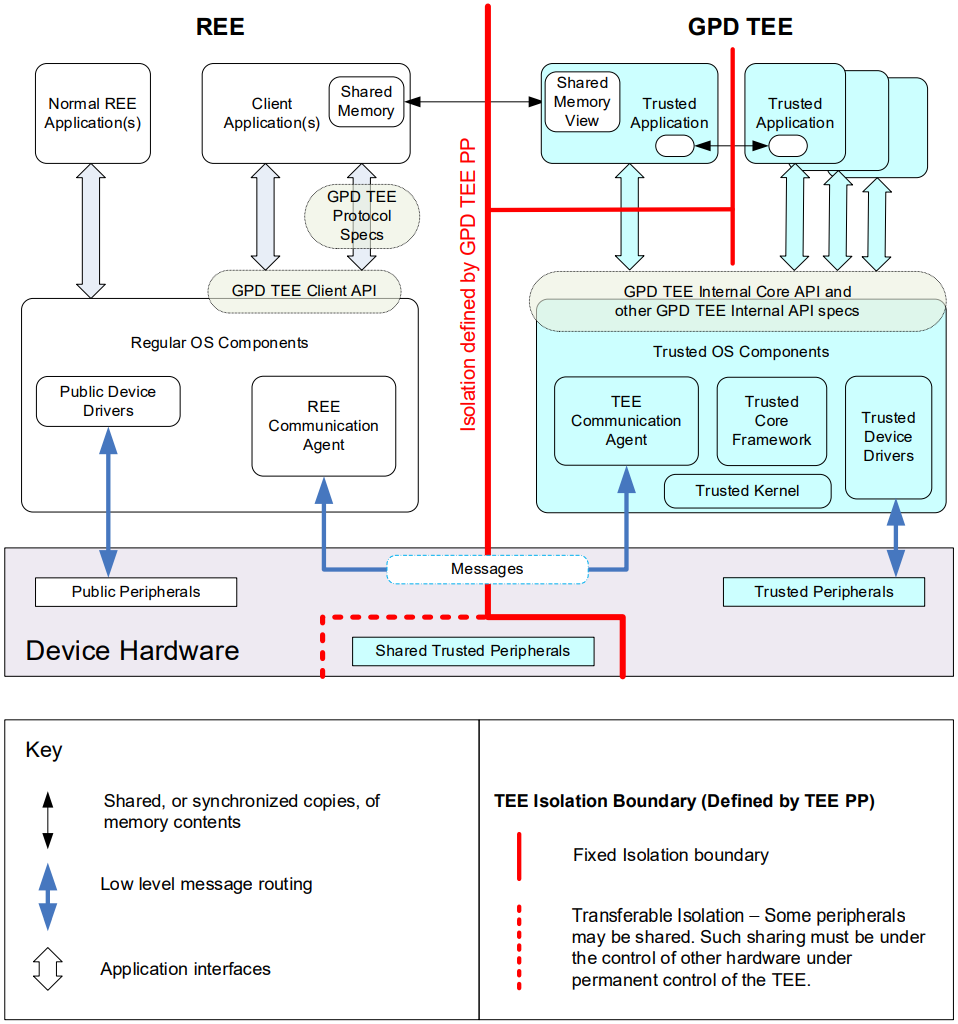
\includegraphics[width=1\textwidth]{immagini/TEE_SW_Architecture}
		\caption{
			Architettura di un TEE conforme GlobalPlatform. 
			Da \textit{TEE System Architecture v1.3 (pag. 28)}
			\cite{gp2020systemarchitecture}
		}
		\label{fig:tee-architecture}
	\end{figure}
	
	\bigbreak
	
	In \figurename~\ref{fig:tee-architecture} si può vedere un possibile esempio di architettura software di un sistema conforme GlobalPlatform. Si può vedere la separazione di REE e TEE, in quanto ambienti completamente separati, dotati ciascuno di sistema operativo, scheduling e risorse proprie.
	
	Le applicazioni all'interno del REE vengono classificate come \textit{Client Applications} (CA), mentre le applicazioni all'interno del TEE sono denominate \textit{Trusted Applications} (TA).
	
	All'interno del TEE è presente un \textit{Trusted Kernel} che fornisce scheduling ed altre funzioni di gestione del sistema operativo, sia per le TA che per il Trusted Core Framework.
	
	\bigbreak
	
	Una CA per richiedere un servizio da una Trusted Application utilizza la \textit{Client API}. Tale API consente di stabilire una sessione con la TA e inviare un messaggio contenente la funzione da invocare e i relativi parametri.
	
	All'interno di entrambi gli ambienti sono presenti dei \textit{Communication Agent}. Questi agenti si occupano di fornire il supporto per lo scambio di messaggi tra la Client Application e la Trusted Application e, se necessario, anche tra diverse TA.
	
	
	\paragraph{Trusted Core Framework:} le Trusted Application possono fare uso della \textit{Trusted Core Framework API}, la quale definisce API ed infrastrutture simili a quelle presente in un sistema operativo. Ciò permette di avere un'interfaccia comune per le TA, indipendentemente dal TEE sulla quale vengono eseguite. Queste specifiche sono contenute all'interno del \textit{TEE Internal Core API Specification}\cite{gp2020internalapi}.
	
	\paragraph{Periferiche:} vengono suddivise in tre categorie: 
	\begin{itemize}
		\item \textit{Public Peripherals}: possono essere utilizzate sia dal TEE che dalle applicazioni REE. L'accesso dalle TA avviene attraverso API fornite dal TEE. L'utilizzo da parte di applicazioni esterne al TEE segue le modalità di accesso standard del sistema operativo.
		\item \textit{Trusted Peripherals}: l'accesso a questo periferiche è consentito esclusivamente a TA autorizzate, tramite interfacce API definite dal TEE.
		\item \textit{Shared Trusted Peripherals}: di norma l'accesso a queste periferiche è consentito solo al TEE, ma questo può concedere temporaneamente l'accesso anche al REE. Il processo di condivisione deve essere comunque gestito da hardware sotto il controllo del TEE.
	\end{itemize}
	
	
	\subsection{Garanzie di Sicurezza}
	\label{subsec:garanzie}
	Come già detto in precedenza, il termine "Trusted Execution Environment" può fare riferimento ad una moltitudine di prodotti, quindi questi potrebbero variare in termini di garanzie di sicurezza che forniscono. Per questo motivo GlobalPlatform ha definito all'interno del \textit{Protection Profile} \cite{gp2020protectionprofile} i requisiti minimi di sicurezza che un TEE deve avere per poter essere certificato. Nonostante le proprietà indicate rappresentino una linea base minima, non è detto che un TEE non possa implementarne altre.
	
	\bigbreak
	
	In generale si può affermare che un TEE dovrebbe garantire le proprietà di integrità e confidenzialità del codice e di ciò che esso crea, e garantire esecuzione isolata rispetto al REE.
	
	Come già visto per altri documenti, GlobalPlatform non stabilisce implementazioni precise ma fornisce solo delle direttive. Nonostante ciò, all'atto pratico si hanno alcune caratteristiche comuni alla maggior parte dei TEE, come l'utilizzo di firme digitali per l'autenticazione del codice e l'utilizzo di supporto hardware per realizzare l'isolamento.
	
	\bigbreak
	
	\paragraph{Isolamento:} la separazione del sistema in zone isolate al fine di garantire la proprietà di isolamento non è nuova, in quanto già proposta da J.M. Rushby nel 1981 \cite{rushby1981separationkernel}. 
	
	Rushby infatti metteva in evidenza come un sistema distribuito permetta di gestire la sicurezza tramite separazione fisica delle parti e mediazione di funzioni fidate.
	
	Questo concetto può essere esteso ad una singola macchina, la quale viene vista come sistema distribuito di componenti indipendenti, i quali quindi permettono di ritenere le proprietà di sicurezza di un sistema distribuito.
	
	Nel mondo TEE questa idea viene ripresa tramite l'implementazione di un \textit{separation kernel}, l'elemento usato per simulare un sistema distribuito, come evidenziato da Sabt et al \cite{sabt2015tee}. Questo permette la coesistenza di diversi sistemi, con diversi requisiti di sicurezza, sulla stessa piattaforma. Fondamentalmente divide il sistema in partizioni e garantisce isolamento tra di esse, tranne per alcune interfacce controllate.
	
	I requisiti di sicurezza generali del separation kernel si possono trovare all'interno del \textit{Separation Kernel Protection Profile} (SKPP) \cite{spkk2007}, ma si possono riassumere in quattro policy di sicurezza principali: 
	\begin{itemize}
		\item \textit{Data (spatial) separation:} dati all'interno di una partizione non possono essere letti o modificati da altre partizioni.
		\item \textit{Sanitization (temporal separation):} le risorse condivise non devono permettere la fuoriuscita di informazioni ad altre partizioni.
		\item \textit{Control of information flow:} la comunicazione tra partizioni deve sempre essere espressa esplicitamente.
		\item \textit{Fault isolation:} falle di sicurezza in una partizione non devono poter condizionare le altre.
	\end{itemize}
	
	La separazione di servizi importanti e dati sensibili permette di minimizzare la possibile superficie d'attacco di un sistema, in quanto la compromissione di un componente non causa danni alle altre parti del sistema. L'unica eccezione sarebbe un fallimento del separation kernel stesso, che per questo motivo deve rimanere più semplice possibile. 
	
	Nella pratica il sistema distribuito descritto da Rushby consiste di due sole componenti, REE e TEE, in quanto tutte le implementazioni effettive prevedono un solo TEE.
	
	\newpage
	
	\paragraph{Integrità e autenticità:} i benefici di protezione durante l'esecuzione dati dall'isolamento vengono annullati se non sono garantite integrità ed autenticità del codice, in quanto modifiche a dispositivo spento permetterebbero la compromissione del sistema.
	
	\bigbreak
	
	Per effettuare questa verifica è necessario un \textit{TEE Secure Boot}, come definito dal \textit{TEE System Architecture} \cite{gp2020systemarchitecture}. Questo è un processo di autenticazione di tutto il software che andrà dentro al TEE, ad eccezione del primissimo codice eseguito per il boot, scritto su una memoria ROM, impossibile da sovrascrivere, la cui integrità è quindi intrinsecamente garantita.
	
	\bigbreak
	
	Ogni componente caricato permette di verificare e caricare il componente successivo, come mostrato in \figurename~\ref{fig:tee-secure-boot}. La verifica può essere implementata, ad esempio, tramite un meccanismo di autenticazione basato su coppie di chiavi, che permettono di firmare e verificare l'hash del codice da caricare. Questo permette di garantire che un ente fidato abbia approvato quel software.
	
	Il firmware del dispositivo deve però conoscere le chiavi pubbliche necessarie per poter verificare la firma dei software da caricare, ma si tratta di un dettaglio implementativo dipendente dal sistema.
	
	\bigbreak
	
	Prima di uscire dal processo di boot il firmware può verificare il boot loader del REE prima della sua esecuzione. In caso di fallimento di verifica di qualsiasi dei componenti prima di questo generalmente il dispositivo termina il processo e viene riavviato, altrimenti continua con l'esecuzione del REE boot loader.
	
	\bigbreak
	
	Questo processo non è dissimile da quello di un \textit{Secure Boot} tradizionale, con le differenze che in un TEE questo processo non termina con l'avvio del sistema operativo e non verifica solo il processo, ma anche il software che andrà in esecuzione sul sistema.
	
	\begin{figure}
		\centering
		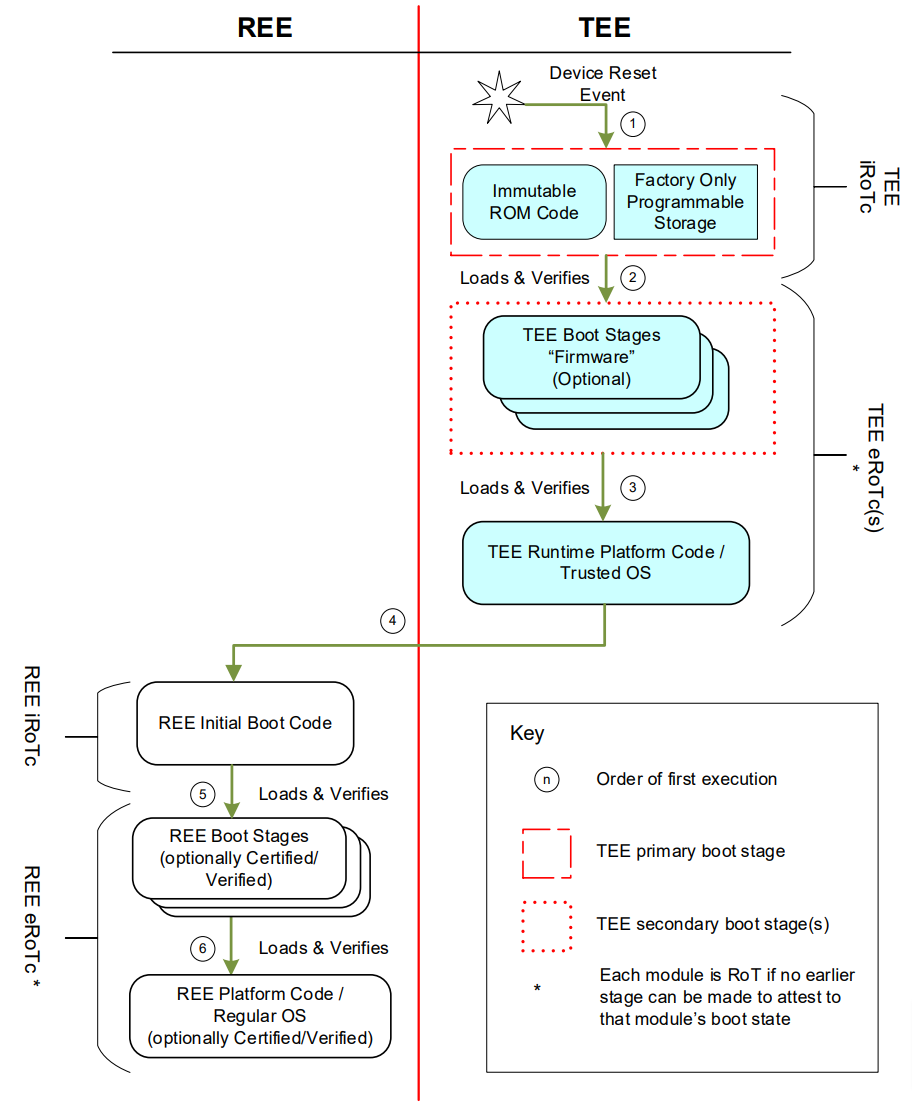
\includegraphics[width=1\textwidth]{immagini/TEE_Secure_Boot}
		\caption{
			Esempio di TEE Secure Boot. 
			Da \textit{GlobalPlatform TEE System Architecture pag. 73}
			\cite{gp2020systemarchitecture}
		}
		\label{fig:tee-secure-boot}
	\end{figure}
	
	\newpage
	
	\section{Applicazioni dei TEE}
	\label{sec:applicazioni}
	I Trusted Execution Environment, grazie alle proprietà di sicurezza che garantiscono, permettono lo sviluppo di nuove applicazioni prima non possibili e l'espansione di quelle già esistenti.
	
	Fino ad ora la maggiore diffusione dei TEE è rimasta in ambito mobile, anche se non sempre pubblicizzati esplicitamente. L'utilizzo non è però limitato a questo settore, le applicazioni dei TEE possono essere molteplici, anche se la maggioranza dei dispositivi non permette l'installazione di software all'interno del TEE dopo la configurazione iniziale.
	
	\bigbreak
	
	Però, tramite l'adozione sempre più vasta degli standard GlobalPlatform e lo sviluppo di TEE open-source come OP-TEE \cite{optee}, si ha una crescente tendenza ad aprire la possibilità a più sviluppatori di implementare i propri TEE e permettere un uso sempre più vasto di questa tecnologia da parte di tutti.
	
	
	\subsection{Archiviazione Sicura}
	\label{subsec:secure-storage}
	Una delle applicazioni più comuni dei TEE è il secure storage, ovvero un meccanismo che consente di proteggere e preservare dati sensibili e critici all'interno di un ambiente altamente affidabile e isolato. Il TEE fornisce una zona sicura all'interno del dispositivo in cui i dati possono essere memorizzati e gestiti in modo sicuro, garantendo la privacy e la riservatezza delle informazioni.
	
	Lo spazio nella maggioranza delle implementazioni è abbastanza limitato e non adatto al supporto di grossi dati strutturati, anche se esistono soluzioni che portano a risultati simili \cite{priebe2018enclavedb} \cite{ribeiro2018dbstore}. Di conseguenza vengono spesso utilizzati per memorizzare sui dispositivi mobili elementi quali chiavi crittografiche, credenziali di autenticazione, certificati digitali, informazioni finanziarie ed altri dati personali.
	
	\bigbreak
	
	L'implementazione Android del secure storage è \textit{Android Keystore} \cite{androidkeystore}, che fa ampio uso del sistema \textit{Trusty TEE} \cite{androidtrustytee}, basato su ARM TrustZone. Questo sistema offre una API per gestire in modo sicuro e protetto le chiavi e i certificati all'interno del TEE, in modo da permettere alle applicazioni di usarlo per operazioni di crittografia, firma digitale e autenticazione.
	
	Inoltre, il sistema Android Keystore offre funzionalità avanzate, come la generazione delle chiavi direttamente all'interno del TEE, senza mai esporle al sistema operativo principale. 
	
	\bigbreak
	
	GlobalPlatform ha definito delle specifiche per la gestione del secure storage, ovvero il \textit{Secure Element Access Control} \cite{gp2020seac}, stabilendo un framework standardizzato per la gestione e protezione dati all'interno del TEE. Un'implementazione comune prevede l'utilizzo di chiavi crittografiche generate e archiviate all'interno del TEE, le quali vengono utilizzate per crittografare i dati sensibili e per proteggere l'accesso al secure storage.
	
	\bigbreak 
	
	Inoltre ci sono alcune implementazioni di \textit{Trusted Platform Module} (TPM) all'interno dei TEE, tramite la funzionalità del Secure Storage. Normalmente il TPM costituisce un componente hardware distinto dal resto del sistema, concepito con obiettivi quali la generazione e la conservazione di chiavi crittografiche, la firma e l'autenticazione sicure, nonché la misurazione dell'integrità del sistema.
	
	Le caratteristiche fisiche e le garanzie di sicurezza offerte da un TPM risultano quindi analoghe a quelle precedentemente descritte per un TEE, mentre l'integrazione del TPM all'interno di quest'ultimo consente di evitare il costo dell'hardware tipicamente richiesto per un chip TPM indipendente.
	
	\subsection{Protezione Contenuti Multimediali (DRM)}
	\label{subsec:drm}
	Nell'era digitale, l'accesso, la distribuzione e la protezione dei contenuti digitali sono diventati elementi cruciali per le industrie dell'intrattenimento, dei media e delle comunicazioni. Tuttavia, con l'aumento della pirateria e delle violazioni dei diritti d'autore, è diventato essenziale sviluppare soluzioni di Digital Rights Management (DRM) sempre più sofisticate per garantire la sicurezza dei contenuti e proteggere i diritti dei creatori e dei detentori dei contenuti stessi.
	
	\bigbreak
	
	Per questo motivo l'utilizzo di sistemi come \textit{Widevine} \cite{widevine} e \textit{PlayReady} \cite{playready} permette di sfruttare l'ambiente TEE (con il loro più alto livello di protezione) per funzionalità quali cifratura del flusso video, verifica delle licenze digitali, autenticazione del dispositivo e protezione contro la copia non autorizzata. Permette anche di mostrare a schermo il video senza che altre applicazioni esterne al TEE possano leggerne i contenuti, a patto che sia presente un canale di comunicazione fidato tra TEE e display, quindi indipendente dal resto del sistema.
	
	Questo permette di garantire che i contenuti video siano accessibili solo da dispositivi e applicazioni autorizzati, proteggendo così i diritti dei detentori dei contenuti e i loro partner di distribuzione. 
	
	\subsection{Garanzie di Sicurezza nel Cloud Computing}
	\label{subsec:protezione-cloud}
	Il cloud computing è un modello di erogazione servizi informatici il quale consente l'accesso on-demand a tramite Internet, senza la necessità di gestire fisicamente l'infrastruttura e sfruttando le risorse richieste in modo estremamente efficiente e scalabile.
	
	Con questo modello sorgono però altre problematiche di sicurezza; ad esempio, il cloud provider deve poter gestire la macchina in quanto mantenitore dell'infrastruttura, ma questo significa anche che ha la capacità di poter leggere tutti i dati presenti in memoria.
	
	Inoltre un elemento fondamentale alla scalabilità del modello è l'utilizzo di una sola macchina fisica per molteplici macchine virtuali (VM), possibilmente assegnate ad altrettanti clienti. Questo significa che più clienti condividono la stessa memoria fisica, aprendo la porta a possibili attacchi che eludono le misure messe in atto per l'isolamento di una VM dalle altre, come già successo \cite{vmescape1} \cite{vmescape2} \cite{vmescape3}. In questo modo gli attaccanti avrebbero modo di accedere ai dati presenti all'interno delle altre macchine virtuali ed in alcuni casi anche di manipolare il codice per i loro scopi.
	
	\bigbreak
	
	In un tale ambiente è normale che un'organizzazione possa ricercare metodi per garantire che il codice eseguito in remoto sia effettivamente quello desiderato. I TEE permettono di implementare sistemi di attestazione remota del codice, generalmente realizzati tramite una TA o meccanismi hardware che generano un report firmato digitalmente sullo stato di esecuzione della macchina. La chiave privata rimane solamente all'interno del TEE, garantendone la sicurezza.
	
	\subsection{Altri Usi}
	\label{subsec:altri-usi}
	Oltre alle applicazioni precedentemente menzionate, i TEE hanno stimolato proposte e trovato impieghi in una vasta gamma di settori, abbracciando un'ampia varietà di utilizzi e applicazioni.
	
	\bigbreak
	
	Nel mondo IoT ci sono state proposte decentralizzare la gestione dei dati utilizzando TEE e smart contract \cite{iotblockchain}. L'idea è quella di un sistema in cui i permessi di accesso vengono applicati tramite smart contract, memorizzando la cronologia di eventi di accesso ai dati nella blockchain. In questo modo le interazioni non necessitano di un sistema centralizzato, in quanto gli smart contract permettono a più parti di specificarne le regole. Infine fornisce un framework che memorizza l'hash dei dati nella blockchain e archivia i dati grezzi all'interno del TEE.
	
	\bigbreak
	
	Un altro esempio è l'implementazione di un protocollo Vehicle-to-Vehicle (V2V) che permette di fornire autenticazione, privacy e resistenza alla manomissione ad i collegamenti tra veicoli a guida autonoma \cite{teeuses_vehicles}. In questo modo, tramite l'utilizzo dei TEE, si previene l'intercettazione e manomissione dei dati, pur mantenendo l'efficienza e scalabilità necessarie per un sistema tale.
	
	\newpage
	
	\section{Implementazioni Hardware per i TEE}
	\label{sec:supporto-hw}
	Affinché un TEE possa soddisfare le proprietà di sicurezza necessarie, è fondamentale che esso disponga di un supporto hardware adeguato. Ad esempio, un requisito critico che necessita tale sostegno è la proprietà di isolamento rispetto al resto del sistema.
	
	Esistono molteplici soluzioni per implementare queste proprietà, perciò in questo capitolo verranno esplorate brevemente alcune delle principali proposte sul mercato.
	
	\subsection{Intel SGX}
	\label{subsec:sgx}
	Intel Software Guard Extensions (SGX) è un'estensione dell'architettura x86 sviluppata da Intel per introdurre un ambiente di esecuzione protetto all'interno dei processori. Viene introdotta nel 2015 con la sesta generazione di processori Intel Core.
	
	SGX consiste in un insieme di istruzioni hardware e strutture di memoria che consentono la creazione e l'isolamento di \textit{enclavi} sicure all'interno del processore, ovvero zone di memoria di dimensione ridotta crittografate e protette tramite meccanismi hardware. 
	
	Per l'accesso a queste zone di memoria è necessario utilizzare i nuovi metodi introdotti da SGX, come ad esempio l'istruzione \texttt{ECREATE} permette di creare un'istanza di enclave, mentre l'istruzione \texttt{ECALL} consente alle applicazioni di interagire con il codice all'interno dell'enclave in modo controllato e sicuro. 
	
	Le istruzioni introdotte sono comparabili a quelle per il passaggio da user mode a kernel mode. Le enclavi vengono sempre eseguite al ring 3 di privilegio (il più basso) ed utilizzano la traduzione degli indirizzi fornita da kernel e hypervisor.
	
	\bigbreak
	
	Come descritto da \cite{sgx_explained}, all'avvio del sistema SGX riserva una porzione di memoria designata come \textit{Processor Reserved Memory} (PRM). Tale area di memoria risulta inaccessibile a tutte le richieste di accesso che non sono riconducibili a un contesto di enclave. Questo ambito di restrizione si estende anche ad elementi quali kernel, hypervisor, System Management Mode (SMM) e Direct Memory Access (DMA).
	
	All'interno di questa zona di memoria si possono trovare la \textit{Enclave Page Cache} (EPC), ovvero pagine di 4KB contenenti codici e dati delle enclavi, oltre all'\textit{Enclave Page Cache Map} (EPCM), la quale viene utilizzata dalla CPU per tracciare lo stato delle pagine all'interno dell'EPC, permettendo di garantire che ciascuna pagina appartenga ad una sola enclave. Quest'ultima è sempre inaccessibile, indipendentemente dal livello di privilegio.
	
	\bigbreak
	
	Un'enclave viene creata tramite l'istruzione \texttt{ECREATE}, la quale inserisce in una pagina libera dell'EPC la \textit{SGX Enclave Control Structure} (SECS). Quest'ultima andrà a contenere informazioni di controllo e metadati relativi all'enclave stessa, come dimensione, base address ed altre proprietà. L'identità di un'enclave è strettamente legata alla sua SECS, in quanto la entry che identifica l'enclave all'interno della EPCM punta alla SECS della stessa. Il sistema usa l'indirizzo virtuale della SECS per identificare l'enclave quando vengono utilizzate istruzioni di SGX.
	
	In seguito il sistema utilizza l'istruzione \texttt{EADD} per caricare codice e dati iniziali all'interno dell'enclave. I dati vengono letti da una struttura chiamata \textit{Page Information} (PAGEINFO), la quale contiene l'indirizzo della pagina EPC da allocare e l'indirizzo della pagina sorgente che andrà copiata nella EPC.
	
	In seguito ad aver caricato i dati necessari, il sistema deve usare una \textit{Launch Enclave} (LE) per ottenere una \textit{EINIT Token Structure}. Tramite l'istruzione \texttt{EINIT} ed il token generato la SECS in questione viene segnata come inizializzata.
	
	Alla fine del processo di vita di un'enclave l'istruzione \texttt{EREMOVE} permette la deallocazione delle pagine utilizzate dall'enclave all'interno della ECP.
	
	La LE è un'enclave privilegiata fornita da Intel, firmata con una chiave presente nell'implementazione di SGX quindi esente dal richiedere un EINIT Token. Questa permette di verificare l'identità di un'enclave in fase di creazione e necessita di informazioni quali chiave di crittografia dell'enclave, politiche di protezione, ecc.
	
	\bigbreak
	
	A partire dai processori di undicesima e dodicesima generazione Intel SGX è stato deprecato sui processori Intel Core, ma continua lo sviluppo per i processori Xeon, comunemente utilizzati in ambito cloud e server.
	
	\subsection{AMD SEV}
	\label{subsec:sev}
	AMD Secure Encrypted Virtualization è una tecnologia introdotta nel 2016 come estensione dell'architettura x86 progettata per offrire isolamento per la memoria di macchine virtuali (VM). Anche se comunemente l'hypervisor viene considerato un componente fidato nel modello di sicurezza della virtualizzazione, tuttavia può non essere sempre così, come ad esempio in ambiente cloud, dove i clienti potrebbero volere una maggiore confidenzialità dei loro dati, normalmente accessibili al service provider.
	
	Al fine di risolvere questo problema AMD SEV permette di crittografare in modo granulare la memoria associata a una specifica macchina virtuale, conferendole un livello di inaccessibilità anche per l'hypervisor stesso. Ogni VM possiede la sua chiave di crittografia unica. La cifratura dei dati in memoria è affidata ad un chip hardware AES-128. Esiste la possibilità da parte della VM di condividere determinate pagine con l'hypervisor.
	
	In aggiunta, sulla scheda madre, trova posto un processore ARM denominato \textit{Secure Processor} (SP), contenente un firmware proprietario. Questo componente assume responsabilità diverse, tra cui la gestione delle chiavi crittografiche. Inoltre fornisce delle API che l'hypervisor deve utilizzare per gestire le chiavi.
	
	\bigbreak
	
	Il SP permette anche un processo di attestazione remota, per aver modo di verificare che le VM in esecuzione presenti in un ambiente remoto siano effettivamente quelle desiderate e che queste siano all'interno dell'ambiente corretto. Viene generato un report contenente tutte le informazioni necessarie per verificarlo, come ad esempio dati iniziali della macchina e policy di sicurezza applicate. In seguito viene firmato tramite una chiave privata presente solamente all'interno del processore, la quale corrispondente pubblica viene fornita da AMD per verificare l'attendibilità del report.
	
	\bigbreak
	
	Partendo da una nuova VM, prima di andare in esecuzione con SEV, questa passa da tre stati, il primo dei quali è UNINIT. In questa fase, con il supporto dell'hypervisor, viene effettuato lo scambio di chiavi con il SP (di tipo ECDH). 
	
	Una volta terminato passa allo stato LUPDATE, nel quale vengono caricati e crittografati i dati da inserire all'interno della VM. Al termine di questo viene calcolato un HMAC per verificare che i dati iniziali non sono stati modificati e passa allo stato LSECRET.
	
	Questo stato permette di passare dati già criptati, quindi che necessitano confidenza più elevata, alla VM. Rimane l'hypervisor come intermediario, che però non può effettuare modifiche/azioni significative con i dati passati. 
	
	Al termine di questo stato la macchina virtuale può andare in modalità di esecuzione regolare.
	
	\bigbreak
	
	In seguito AMD ha rilasciato versioni aggiornate di SEV, la prima delle quali nel 2017: SEV-ES (Encrypted State) \cite{sev_es}, incentrata sulla crittografia dello stato dell'architettura delle CPU, criptando anche registri interni, page table e altre strutture interne. Prima di questo SEV salvava in chiaro i registri di una VM dopo un context switch con l'hypervisor.
	
	Nel 2021 viene rilasciata SEV-SNP (Secure Nested Paging) \cite{sev_snp}, introdotta per migliorare la sicurezza nelle architetture di multi-tenant e cloud. Introduce una nuova tabella di pagine crittografata all'interno di ogni VM che garantisce l'isolamento tra VM diverse. Le VM non possono accedere alle tabelle di pagine l'una dell'altra.
	
	\newpage
	
	\subsection{Arm TrustZone}
	\label{subsec:trustzone}
	ARM TrustZone è una tecnologia di sicurezza introdotta nel 2004 e integrata nei processori ARM, che sono ampiamente utilizzati in dispositivi mobili, dispositivi IoT (Internet of Things) e altri sistemi embedded. L'obiettivo principale di TrustZone è creare un ambiente sicuro all'interno di un singolo processore, in modo che diverse parti del sistema possano operare in modalità sicura o non sicura, a seconda delle esigenze, senza compromettere la sicurezza dei dati e delle operazioni.
	
	TrustZone divide il processore in due mondi distinti: "\textit{Secure}" e "\textit{Non-Secure}", i quali operano in parallelo, con risorse distinte per ogni ambiente e separate in modo hardware. Questo fornisce un ambiente in cui è possibile eseguire software critico e operazioni di sicurezza in modo isolato dal resto del sistema.
	
	All'interno di ARM sono presenti 4 livelli di privilegio, da EL0 (più basso) a EL3 (più alto). Il livello più alto viene utilizzato dal sistema per il passaggio da mondo \textit{Secure} e \textit{Non-secure}. Questo livello rappresenta il \textit{separation kernel} descritto precedentemente (\ref{subsec:garanzie}).
	
	Il software che gestisce il passaggio, sui processori serie Cortex-A, è chiamato "\textit{Secure Monitor}". Sui dispositivi dotati di Cortex-M non è presente in quanto il passaggio da un mondo all'altro è implementato direttamente all'interno della logica del processore. In entrambi i casi si ha una separazione completa e garantita a livello hardware.
	
	\bigbreak
	
	Il processore può trovarsi in solo uno dei mondi e lo stato attuale può essere rilevato tramite un nuovo bit presente sul bus dati, il \textit{Non-Secure} (NS) bit. Quest'ultimo può essere letto tramite il \textit{Secure Configuration Register} (SCR), il quale contiene vari flag e bit che controllano il comportamento del sistema. 
	
	Inoltre il firmware deve implementare un modo per gestire la \textit{Secure Monitor Call} (SMC), l'istruzione che permette di entrare in "\textit{monitor mode}" e cambiare la modalità del processore. Funziona similmente ad una system call: quando chiamata tramite il suo codice specifico passa al livello di privilegio EL3 e invoca un handler implementato nel firmware, all'interno della tabella degli interrupt del processore.
	Il firmware a livello EL3 è anche incaricato di caricare i sistemi operativi del mondo sicuro e normale.
	
	
	\bigbreak
	
	TrustZone estende anche l'infrastruttura di memoria con alcune funzionalità di sicurezza, in particolare: \textit{TrustZone Address Space Controller} (TZASC) e \textit{TrustZone Memory Adapter} (TZMA).
	
	Il TZASC permette partizionare la DRAM e marcare specifiche regioni di memoria come sicure o non-sicure, in modo che applicazioni nel secure world possano accedere alle regioni associate al mondo normale, ma non in contrario. Il TZMA effettua una funzione simile ma su altre memorie come ROM o SRAM.
	
	Queste componenti sono opzionali, quindi la loro presenza e la granularità al quale possono agire dipende dall'implementazione.
	
	\bigbreak 
	
	All'interno di TrustZone non viene effettuata nessuna verifica dell'integrità del codice all'avvio, onere lasciato ai produttori.
	
	Una soluzione comune è avere una coppia di chiavi pubblica e privata, presenti all'interno del chip. Il codice viene caricato assieme ad un suo hash, firmato con la chiave pubblica e poi il tutto viene confrontato con la chiave stampata nel chip.
	
	\begin{figure}[t]
		\centering
		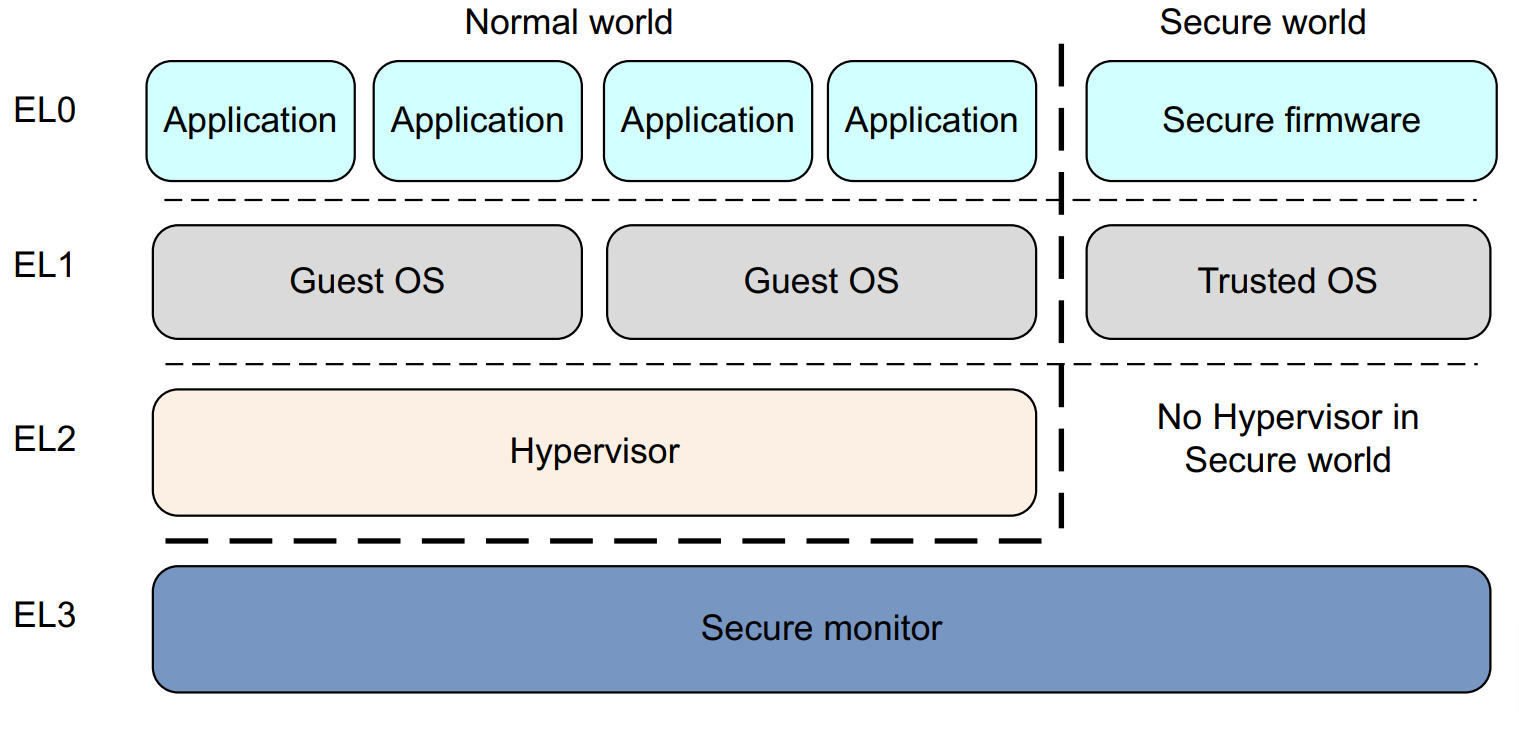
\includegraphics[width=0.8\textwidth]{immagini/ARM_TZ_Levels}
		\caption{
			Livelli di privilegio di ARM TrustZone. Da \textit{"ARM Cortex-A Series Programmer's Guide for ARMv8-A"}
			\cite{arm_programmers_manual}
		}
		\label{fig:arm-exception-levels}
	\end{figure}
	
	\subsection{TEE RISC-V}
	\label{subsec:riscv}
	RISC-V è un Instruction Set Architecture (ISA) sviluppato principalmente dall'Università della California, Berkeley, negli Stati Uniti. Il progetto è nato nel 2010 per poi coinvolgere anche contributori volontari non affiliati all'università. Nel 2015 viene fondata la RISC-V Foundation, creata con il fine di sostenere e promuovere lo sviluppo e l'adozione dell'architettura RISC-V.
	
	Diversamente da molti altri ISA, RISC-V è sviluppato sotto licenza open source, quindi l'utilizzo è gratuito. Questo, oltre al buon supporto da parte di toolchain e sistemi operativi, ha permesso di far crescere notevolmente nel tempo l'adozione di RISC-V, coinvolgendo una vasta comunità di aziende, istituti di ricerca e sviluppatori indipendenti. 
	
	La possibilità di avere a disposizione uno stack software senza doverlo scrivere da zero o pagare licenze ha reso RISC-V un ambiente interessante per sviluppare hardware, anche in ambito TEE.
	
	\bigbreak
	
	Data la flessibilità dell'hardware, i progetti esistenti generalmente si concentrano sulla possibilità di creare TEE che rispondano alle proprie esigenze. Per citare alcuni di questi progetti, Penglai \cite{penglai} e Keystone \cite{keystone}. 
	
	Le soluzioni esistenti, citate nelle sezioni precedenti, pongono limiti progettuali che possono rendere difficoltoso utilizzare l'ambiente in un modo che sia in linea con le proprie esigenze, a volte forzando gli sviluppatori a creare soluzioni alternative, come ad esempio nel caso di dover eseguire applicazioni non modificate all'interno di SGX \cite{grapheneSGX}.
	
	Entrambi i progetti citati precedentemente si basano sullo sfruttare l'isolamento della memoria fornita da RISC-V, chiamata \textit{Physical Memory Protection} (PMP), per ottenere zone di memorie protette da accessi non autorizzati. Utilizzano la \textit{machine mode} (il livello di privilegio più alto di RISC-V) per eseguire un secure monitor con il compito di separare l'ambiente di esecuzione ordinario dalle enclavi sicure create.
	
	L'idea è simile a quelle presentate precedentemente con TrustZone o SGX, ma con minori limiti alla memoria e più possibilità di configurare le enclavi.
	
	\subsection{Processori Dedicati}
	\label{subsec:altri-rpc}
	Un possibile metodo per integrare un TEE all'interno di un dispositivo è quello di avere un secondo processore collegato solamente alle componenti fidate del sistema. Questa soluzione risulta più costosa, ma si hanno alcuni esempi, in particolare su dispositivi mobili di fascia alta.
	
	\bigbreak
	
	A partire dal Pixel 3 Google ha incluso all'interno dei suoi telefoni anche processori della serie \textit{Titan M}, basati sull'architettura RISC-V, i quali sono sistemi a tutti gli effetti, contenenti la propria memoria, RAM, acceleratore crittografico e sistema operativo. L'area TrustZone, anch'essa presente, viene utilizzata solamente come ponte per interagire con il chip \textit{Titan M}.
	
	Alla base, questo processore è stato pensato come metodo per incrementare le misure di sicurezza standard di Android, normalmente affidate ad un TEE presente sul \textit{System on a Chip} (SoC) principale. Permette quindi di immagazzinare dati sensibili come chiavi crittografiche e dati biometrici, oltre che supportare il processo di Secure Boot e validare la versione di Android in esecuzione.
	
	\bigbreak 
	
	Apple include nei propri dispositivi un sottosistema chiamato \textit{Secure Enclave}. Esegue funzionalità simili agli altri TEE, permettendo di implementare funzionalità come \textit{Apple Pay} e \textit{Touch ID}. Si tratta di un SoC che esegue una versione modificata del kernel L4, un sistema molto ridotto, con l'aggiunta di servizi e driver proprietari. Inoltre è collegato a periferiche proprie, accessibili tramite MMIO, come acceleratore crittografico e generatore di numeri casuali.
	
	\section{Vulnerabilità Note}
	\label{sec:vulnerabilità}
	Per quanto incentrati sulla sicurezza i TEE non sono completamente esenti da vulnerabilità. Nel tempo sono stati trovati diversi attacchi che permettono di aggirare le misure di sicurezza offerte da questi sistemi.
	
	\bigbreak 
	
	La cache permette di porre molti dubbi riguardo la sicurezza del codice all'interno di un processore, in quanto si tratta di un vettore d'attacco comune a più soluzioni hardware. SGX, TrustZone e SEV ne sono risultati suscettibili. Nonostante queste soluzioni rendano generalmente inaccessibili i dati tramite metodi convenzionali, la cache può spesso essere vittima di attacchi side channel.
	
	Sfruttando attacchi basati sul \textit{timing} della cache, \textit{ARMageddon} \cite{armageddon} ha permesso l'ottenimento di dati tramite attacchi come \textit{Prime+Probe}, \textit{Flush+Reload}, \textit{Evict+Reload} e \textit{Flush+Flush}, già visti su altre tipologie di processori, raggiungendo un elevato livello di precisione e risoluzione, fino a monitorare l'attività all'interno della cache di TrustZone. All'interno del testo vengono presentate, e risolte, le problematiche poste da ARM per queste tipologie di attacco, come l'eterogenea composizione delle cache e la mancanza di un'istruzione dedicata al flush. Vengono proposte anche possibili contromisure software per, se non impedire, rendere più difficoltoso l'attacco. Un attacco simile viene presentato da \textit{CacheZoom} \cite{cachezoom}, ma sfruttando le vulnerabilità di SGX.
	
	Un altra tipologia di attacco trovato alla cache di ARM \cite{aliasdriven} sfrutta possibili configurazioni errate della memoria, le quali permettono ad un attaccante di mappare molteplici indirizzi virtuali ad uno stesso indirizzo fisico, con politiche di memoria incoerenti, ed osservare in che livello della cache questi vengono inseriti. Questo permette di arrivare ad infrangere la confidenzialità dei dati posti in memoria sicura.
	
	Un altro modo per sfruttare incoerenze della cache è \textit{CacheKit} \cite{zhang2016cachekit}. Su ARM la separazione delle linee della cache tra TrustZone e mondo normale non permette al mondo sicuro di accedere alla cache del mondo normale. Queste incoerenze possono portare a nascondere la presenza di un rootkit. Il codice rimane nella cache del mondo sicuro, ma non in memoria, permettendo di rimanere invisibile dal normal world.
	
	Su AMD SEV invece sono stati trovati problemi con la gestione del Translation Lookaside Buffer (TLB) \cite{li2021tlb}, permettendo poisoning di questa cache. L'estensione su SEV del TLB contiene diverse vulnerabilità che lo rendono non sicuro per il tipo di minacce che SEV stesso si presuppone di prevenire. Infatti l'hypervisor potrebbe essere in grado di effettuare attacchi di TLB Poisoning, con lo scopo di compromettere integrità e confidenzialità delle VM utilizzanti SEV.
	
	\bigbreak 
	
	Da non sottovalutare anche all'interno dei TEE la possibilità di attacco tramite vulnerabilità del software, come possono essere la mancata validazione degli input e l'overflow di memoria. Queste sono le stesse che si possono presentare in qualsiasi altro software e prevedono le stesse contromisure, ovvero tutte le \textit{best practices} per la sicurezza del software.
	
	Un esempio di attacco di questo tipo è stato trovato per il chip Titan M di Google \cite{attack_titanM}. Si tratta di un errore nella copia di un buffer all'interno dell'implementazione per Pixel di Keymaster, il quale permetterebbe di scrivere un byte di memoria in una zona arbitraria. Questo, assieme alla memoria statica del Titan M, permette di estrarre informazioni sicure del TEE.
	
	
	Inoltre, in particolare facendo riferimento ad ARM, la superficie d'attacco visibile all'interno di una TA generalmente è abbastanza estesa, ad esempio è presente una grande quantità di chiamate di sistema del kernel TEE a cui può avere accesso ed in alcuni sistemi una TA può andare a mappare in qualsiasi zona del sistema operativo ospitante. Una vulnerabilità all'interno di una TA può quindi portare al controllo completo del sistema.
	
	\bigbreak
	
	Per migliorare i consumi ed il calore generato dai processori esistono tecniche che modificano i valori di frequenza e voltaggio del processore in base al carico di lavoro. Per fare ciò molti processori espongono interfacce privilegiate. Si possono sfruttare queste interfacce per minare la sicurezza del sistema, tramite dei \textit{fault attacks}. Siccome il processore può funzionare correttamente solo in un determinato range di frequenza e voltaggio si può indurre l'hardware a commettere errori, voluti e predeterminati, al fine di estrarre informazioni sensibili.
	
	Sono stati trovati attacchi di questo tipo all'interno di SGX (\textit{Plundervolt} \cite{plundervolt}), TrustZone (\textit{CLKscrew} \cite{clkscrew}) e SEV (\cite{sev_power_attack}).
	
	Mitigare questi attacchi può non essere semplice, in quanto richiedono aggiornamenti del microcode o modifiche hardware.
	
	\newpage
	
	\section{OP-TEE}
	\label{sec:optee}
	Open Portable Trusted Execution Environment \cite{optee} è un progetto nato nel 2013, anche se sotto un altro nome e come TEE proprietario della ST-Ericsson, per fornire un ambiente di esecuzione open source, sicuro e affidabile per architetture ARM, sfruttando la tecnologia TrustZone, anche se è stato strutturato in modo tale da essere compatibile con altre tecnologie hardware che forniscono le funzionalità di un TEE.
	
	OP-TEE è stato sviluppato per essere compatibile con le specifiche GlobalPlatform, per questo motivo il software presenta caratteristiche architetturali simili (vedi \figurename~\ref{fig:optee-architecture}). Inoltre si tratta di uno dei due TEE per cui è implementato un driver all'interno del sottosistema Linux, oltre ad AMD Platform Security Processor.
	
	\bigbreak 
	
	All'interno di OP-TEE è anche presente un supporto (sperimentale) alla virtualizzazione \cite{optee_virtualization}, il quale permette di avere una singola istanza di OP-TEE in grado di eseguire TA richieste da multiple macchine virtuali. Lo stato relativo ad ogni VM è isolato dalle altre in modo che non possano interagire.
	
	\bigbreak
	
	Per questi motivi si tratta del TEE scelto per il progetto, anche se l'implementazione delle varie componenti non è legata ad un TEE specifico.
	
	\begin{figure}[h]
		\centering
		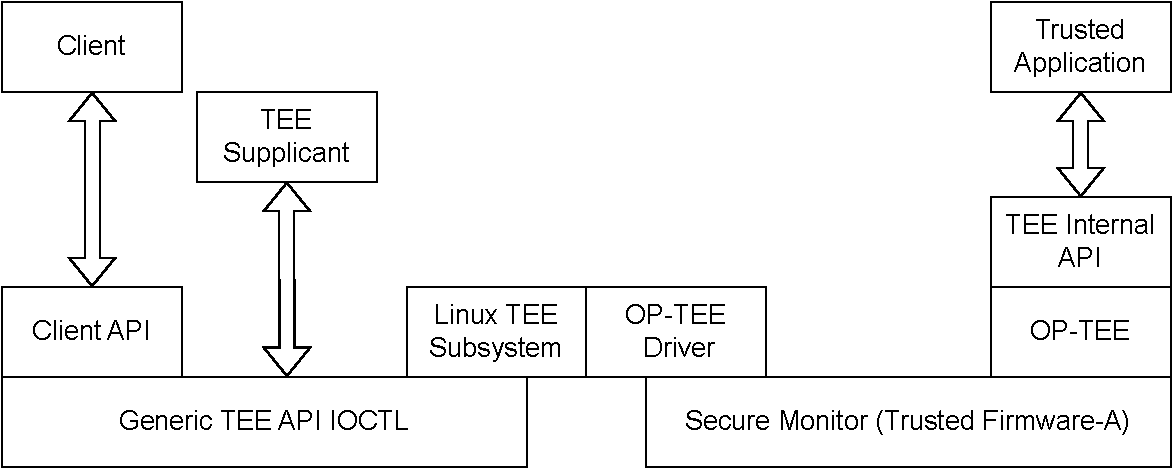
\includegraphics[width=0.8\textwidth]{immagini/optee-system-architecture}
		\caption{ Componenti dell'architettura OP-TEE. Da sinistra verso destra si possono vedere user space, kernel e secure world. Da \textit{"TEE Subsystem - OP-TEE Driver"} \cite{linux_tee_subsystem} }
		\label{fig:optee-architecture}
	\end{figure}
	
	\newpage
	
	\section{ARM CCA} 
	\label{sec:cca}
	Il \textit{Confidential Computing}, ovvero la protezione dei dati durante la computazione, sta assumendo sempre più rilevanza, per questo motivo ARM ha presentato \textit{ARM Confidential Compute Architecture}, con l'obiettivo di impedire l'accesso e la modifica dei dati da parte anche di software privilegiato, come può essere un hypervisor.
	
	\bigbreak
	
	La \textit{Confidential Compute Architecture} introduce un metodo più dinamico e flessibile (rispetto a quelli tradizionali) per la creazione di TEE tramite l'introduzione dei \textit{Realms}. Questi rappresentano una nuova astrazione per proteggere integrità e confidenzialità dei dati.
	
	L'hardware permette la creazione ed il mantenimento di un \textit{Realm World} (RW), uno spazio di indirizzamento fisico dedicato ai Realm, presente in modo ortogonale ai mondi Non-Secure (NS) e Secure precedentemente esistenti. 
	
	Ogni ambiente ha un suo \textit{Physical Address Space} (PAS), ovvero la sezione di memoria che gli viene dedicata. Quest'ultima è gestita dinamicamente e senza limitazioni statiche su quale ambiente può controllare che zona. All'interno della \figurename~\ref{fig:optee-architecture} si può notare come CCA estende la precedente architettura ARM.
	
	\begin{figure}[h]
		\centering
		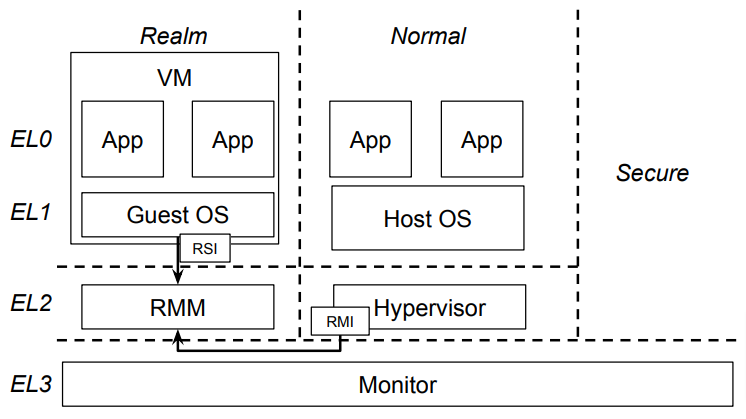
\includegraphics[width=0.7\textwidth]{immagini/CCA_Arch}
		\caption{ Architettura di ARM CCA. Da \textit{Design and Verification of the Arm Confidential Compute Architecture} \cite{arm_cca_presentation}}
		\label{fig:cca_arch}
	\end{figure}
	
	I livelli di privilegio presenti per ognuno dei mondi sono EL0 per gli utenti, EL1 per il kernel e EL2 per l'hypervisor. Realm ne introduce un quarto, EL3, a privilegio più alto, il quale si occupa della transizione da un mondo all'altro.
	
	All'interno di ogni mondo i livelli di privilegio ed il loro funzionamento rimane uguale, ma software all'interno del mondo NS non può accedere a memoria o stati della CPU utilizzati da software nel Realm world.
	
	\bigbreak
	
	CCA introduce il \textit{Realm Management Monitor} (RMM), ovvero codice firmware eseguito nel RW a livello più alto dei Realm (EL2 nel RW). Ha il compito di gestire le richieste proveniente dal NS world riguardo la gestione dei Realm, mantenendo integrità e confidenzialità di quest'ultimi. Il software presente all'interno del NS world ritiene comunque il controllo sulla allocazione dinamica delle risorse hardware riguardanti i Realm. 
	
	Inoltre controlla l'esecuzione dei Realm e li isola tramite tecnologie di virtualizzazione. Dovendo solamente garantire le proprietà di sicurezza di CCA, e non tutte le funzioni tipiche di gestione della virtualizzazione, risulta significativamente più piccolo rispetto ad un tipico hypervisor.
	
	\bigbreak
	
	A livello EL3 viene eseguito il \textit{EL3 Monitor} (EL3M). Ha la responsabilità di effettuare il context switch tra i tre mondi e gestire la \textit{Granule Protection Table} (GPT), la tabella che tiene traccia del PAS di ogni zona di memoria. Solo il EL3M può cambiare il PAS di un \textit{granule} ed aggiornare la voce relativa all'interno della GPT.
	
	Il software presente all'interno degli altri mondi può effettuare una \textit{Secure Monitor Call} (SMC) al EL3M per richiedere un cambio di PAS.
	
	\bigbreak
	
	Si ha fondamentalmente una "delegazione" di zone di memoria da parte dell'hypervisor al RMM, il quale ne garantisce le proprietà di sicurezza. Tutta la memoria utilizzata dall'RMM deve essere prima stata delegata dall'hypervisor.
	
	Per effettuare richieste all'RMM, questo mette a disposizione una \textit{Realm Management Interface} (RMI), dove ogni comando per la gestione dei Realm è implementato come una SMC.
	
	\bigbreak
	
	Ognuno dei 3 mondi presenti può accedere solamente alla propria memoria ed a quella del Non-Secure world, con l'eccezione del software presente a livello EL3, il quale ha accesso completo a tutta la memoria fisica. Il controllo degli accessi viene fatto rispettare tramite supporto di meccanismi hardware.
	
	Questo permette di escludere anche software privilegiato, come hypervisor e sistemi operativi, dall'accesso delle zone di memoria degli altri mondi.
	
	\bigbreak
	
	Si tratta di una tecnologia che permetterebbe di risolvere diversi problemi in ambito di sicurezza cloud, ma non ancora disponibile, sarà presente assieme ad ARMv9-A.
	
	\chapter{TEE in Ambiente Cloud}
	\label{cap:problema}
	%Virttee design problems, problema nel portare roba in cloud e come risolverli. Problematiche e come sono state affrontate. Componenti senza implementazione, mettere schemi di funzionamento
	Il \textit{Cloud Computing} rappresenta la nascita di un nuovo modello di servizi il quale permette di utilizzare un'infrastruttura messa a disposizione da un provider, fornendo un'alternativa flessibile e scalabile all'infrastruttura informatica tradizionale basata su server locali. Il concetto di \textit{Infrastructure as a Service} permette di avere una propria applicazione web senza i costi legati al mantenimento della struttura, lasciati al provider.
	
	\bigbreak
	
	Questo però porta nuove preoccupazioni in termini di sicurezza, in quanto tutti i dati devono essere portati su macchine fisiche al di fuori del proprio controllo. Il provider deve essere in grado di accedere alla macchina in quanto necessario per ottimizzare l'utilizzo delle risorse, ma questo può portare ad avere dubbi su cosa avviene ai dati e chi ne ha accesso una volta in esecuzione.
	
	Ciò che permette la condivisione di risorse su una stessa macchina è la \textit{virtualizzazione}, avere una macchina virtuale per ogni cliente permette di allocare in modo dinamico la potenza di calcolo e di gestire in modo semplice i dati tra una macchina e l'altra. La suddivisione tra i vari clienti viene resa possibile tramite l'hypervisor, il quale controlla le macchine virtuali su un server fisico.
	
	Questo tipo di gestione vuole anche dire che l'hypervisor può avere accesso a tutti i dati delle macchine virtuali e non si hanno garanzie che il provider del servizio sia fidato (seppur sia ragionevole assumerlo nella maggior parte dei casi). Può rappresentare un problema in caso di dati che richiedono una sicurezza maggiore, come può essere nei casi di utilizzo dei TEE.
	
	Un altro aspetto che può rivelarsi problematico è la condivisione dello stesso hardware tra clienti diversi. La separazione dovrebbe essere completa ma nel caso in cui un attaccante riuscisse a prendere il controllo o eludere l'hypervisor sarebbe in grado di accedere e possibilmente alterare i dati di tutti gli altri clienti presenti sulla macchina.
	
	\section{TEE as a Service}
	\label{sec:taas}
	In ambiente cloud potrebbe sembrare una soluzione efficace l'utilizzo di un TEE per garantire integrità e confidenzialità dei dati, ma si presentano alcune difficoltà, in quanto le possibilità di utilizzo dei Trusted Execution Environment all'interno di ambienti virtualizzati risultano limitate. Il modello tradizionale generalmente richiede un TEE dedicato per ogni cliente, il quale dovrebbe essere in grado di gestirlo.
	
	Inoltre non è sempre fattibile per limitazioni tecniche dovute alla condivisione della macchina.
	
	\bigbreak
	
	Per aggirare queste limitazioni tecniche una possibile soluzione sarebbe includere il TEE all'interno del servizio proposto dal provider, permettendo di utilizzare un solo dispositivo fisico per tutti i client presenti sulla macchina. Questo però richiede la condivisione di un singolo TEE con più client virtuali, il che pone alcuni problemi.
	
	Il metodo presentato da Cutecchia \cite{tesi_cutecchia} per implementare la condivisione è l'utilizzo di un device virtuale, inserito come estensione dell'hypervisor, con il ruolo di intermediario tra TEE fisico ed ambiente virtuale. 
	
	\bigbreak
	
	\begin{figure}[h]
		\centering
		\begin{subfigure}{\columnwidth}
			\centering
			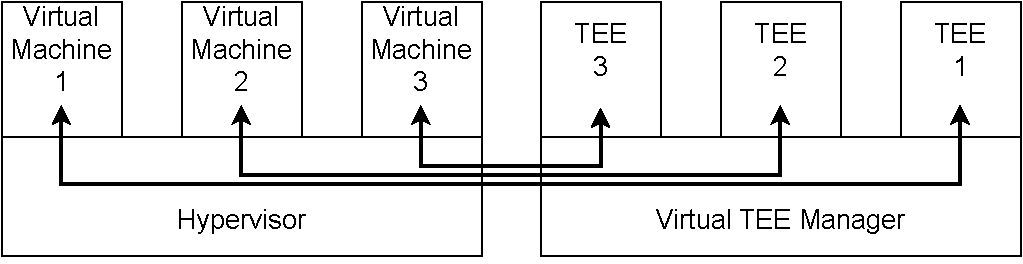
\includegraphics[width=0.8\linewidth]{immagini/common-cloud-tee-model}
			\caption{Il modello tradizionale di TEE in ambiente cloud}
			\label{fig:common-cloud-tee-model}
		\end{subfigure}
		
		\begin{subfigure}{\columnwidth}
			\centering
			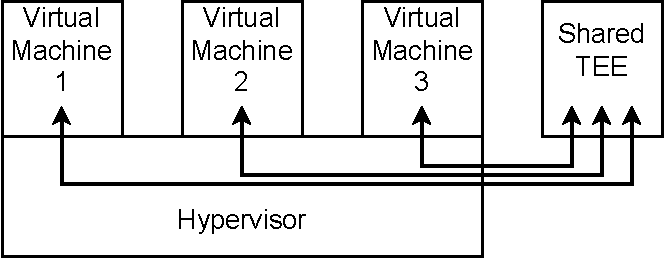
\includegraphics[width=0.53\linewidth]{immagini/our-cloud-tee-model}
			\caption{Il modello descritto, con un TEE condiviso tra più VM}
			\label{fig:our-cloud-tee-model}
		\end{subfigure}
		\caption{Confronto tra i due modelli discussi, da \cite{tesi_cutecchia}}
	\end{figure}
	
	In questo modo il TEE diventa parte del servizio fornito dal provider, semplificandone la gestione e l'utilizzo da entrambe le parti.
	
	\section{Implementazione Passthrough}
	\label{sec:pass_impl}
	Il passthrough è un sistema che consente a una macchina virtuale di inviare richieste al TEE presente sull'host. Per implementarlo è necessario creare un canale di comunicazione tra VM e host, estendendo l'hypervisor (in questo caso QEMU) con un nuovo device virtuale.
	
	Il driver per questo device viene utilizzato all'interno della VM e si interfaccia con il sottosistema TEE e il device virtuale. Il compito del driver è quello di soddisfare le richieste verso il TEE inoltrando e ricevendo le richieste dal device virtuale.
	
	Host e VM comunicano utilizzando questo device e implementano un protocollo di comunicazione a messaggi, i quali rappresentano le richieste che il guest può fare al TEE.
	
	\begin{figure}[h]
		\centering
		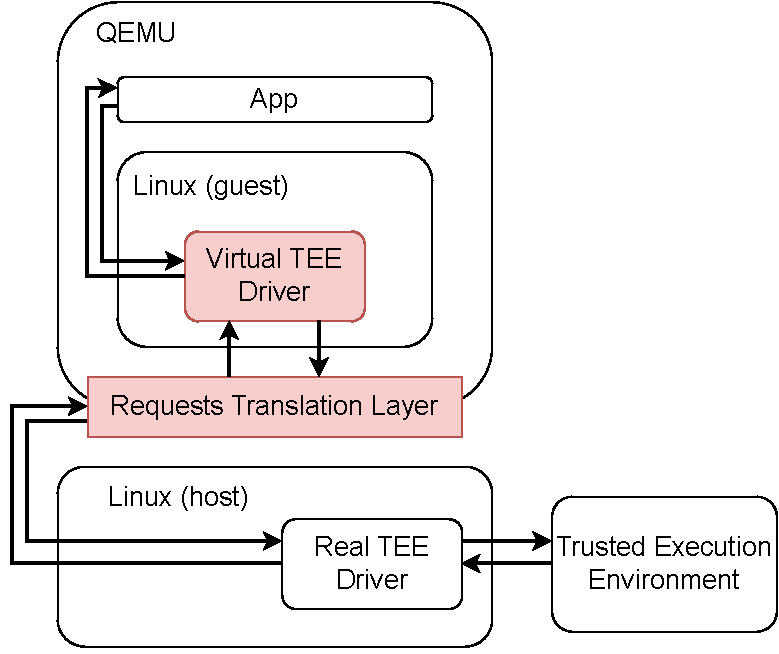
\includegraphics[width=0.7\linewidth]{immagini/tee-passthrough-schema}
		\caption{
			Schema del sistema di passthrough. In evidenza le aggiunte effettuate. Da \cite{tesi_cutecchia}
		}
		\label{fig:passthrough-schema}
	\end{figure}
	
	\paragraph{Device virtuale:} è stato implementato come estensione della macchina ARM \texttt{qemu\_virt\_8}, ma non si tratta di una scelta vincolante. Comunica con il driver tramite Memory Mapped Input/Output (MMIO), l'hypervisor si occuperà di inoltrare il messaggio scritto dal guest.
	
	L'uso del device virtuale è strutturato similmente all'utilizzo dell'interfaccia user-space del sottosistema TEE di Linux \cite{linux_tee_subsystem}. In breve, il driver per aprire la connessione con il TEE deve leggere il valore identificativo della connessione da un registro, con una semantica simile ai descrittori di file. 
	
	Per inviare una richiesta si ha un registro nella quale viene inserito l'indirizzo del buffer di memoria contenente il messaggio. Si ha anche un registro che permette di ottenere informazioni sull'esito della richiesta in seguito all'operazione.
	
	\paragraph{Driver:} è stato implementato come modulo \textit{out-of-tree} del kernel Linux e progettato per contenere il minimo delle funzioni necessarie. Durante il caricamento l'area di memoria del device virtuale viene ri-mappata in una zona di memoria virtuale accessibile al kernel.
	
	Ha il compito di ricevere richieste dal sottosistema TEE, convertirle in messaggi aderenti al protocolli di comunicazione ed inviarli al device virtuale. 
	
	\paragraph{Protocollo:} necessario per la comunicazione tra host e guest, progettato per semplicità e strutturato similmente alle operazioni supportate dai device file TEE reali.
	
	Si basa su un sistema a messaggi. Ogni messaggio presenta una struttura comune che serve per indicare come deve essere interpretato il resto del messaggio.
	
	\begin{figure}[H]
		\centering
		\GeneraSchemaPacchetto{
			type/8}{
			payload\_size/8,
			payload/variabile
		}
		\caption{
			Header dei messaggi del protocollo. Da \cite{tesi_cutecchia}}
		\label{fig:message-wrapper-schema}
	\end{figure}
	
	Il campo \textit{type} permette di identificare il contenuto di \textit{payload}, tramite un set di valori predefiniti. Il campo \textit{payload\_size} indica la dimensione in byte del campo \textit{payload} seguente.
	
	All'interno del payload di molti messaggi è presente un valore \textit{fd} (\textit{File Descriptor}), il quale serve al driver per stabilire a quale connessione tra hypervisor e TEE inoltrare il messaggio. Messaggi parte della stessa connessione presentano lo stesso valore \textit{fd}.
	
	\paragraph{Hypervisor:} l'estensione dell'hypervisor presenta più funzionalità. Come prima cosa, deve implementare il device virtuale, per il quale mantiene uno "stato" dei registri, aggiornato ad ogni scrittura nella zona MMIO del device in modo da sapere quando è necessario gestire un messaggio. Inoltre vengono implementati i messaggi del protocollo.
	
	Astraendo, una delle funzioni è ricevere messaggi ed effettuare le rispettive \texttt{ioctl} e riscrivere nella memoria dell'host il risultato. Il problema con questo risiede nei valori che vengono passati all'hypervisor, in quanto validi solo all'interno della VM. Per risolvere il problema sono state implementate tabelle di traduzione dei valori.
	
	Un altro problema riguarda la condivisione dei buffer di memoria tra TEE e guest, in quanto la memoria fisica non può essere condivisa, quindi sono presenti due buffer separati, uno per il TEE ed uno per il REE, che l'hypervisor si occupa di sincronizzare. I dati vengono copiati da guest ad un buffer accessibile all'hypervisor primo di iniziare una chiamata al TEE, e l'opposto avviene prima di lasciare nuovamente il controllo alla VM. 
	
	\subsection{Performance Passthrough}
	\label{subsec:perf-pass}
	Il passthrough, per sua natura, introduce un overhead aggiuntivo, ma potenzialmente accettabile, in gran parte dato dalla sincronizzazione dei buffer di memoria condivisa. 
	
	All'interno della \tablename~\ref{tab:performance_pass} vengono riportati i tempi di esecuzione di \textit{xtest}, una suite di test presente all'interno di OP-TEE e di una semplice Trusted Application che si occupa in solamente di incrementare un valore.
	
	\begin{table}[h]
		\centering
		1
		\begin{tabular}{cccccc}
			\multicolumn{1}{c|}{}  & \multicolumn{2}{c|}{\textbf{Senza Passthrough}} & \multicolumn{2}{c|}{\textbf{Con Passthrough}} &  \\
			\multicolumn{1}{c|}{\multirow{-2}{*}{\textbf{Test}}} &
			\multicolumn{1}{c|}{\textbf{Media}} &
			\multicolumn{1}{c|}{\textbf{Dev. Std}} &
			\multicolumn{1}{c|}{\textbf{Media}} &
			\multicolumn{1}{c|}{\textbf{Dev. Std}} &
			\multirow{-2}{*}{\textbf{Overhead}} \\ \hline
			\texttt{xtest -l 15}    & 1221,416  & 7,876 & 1319,174 & 12,790 & 8,003\% \\
			\texttt{hello\_world}   & 34,989    & 0.132 & 35.581 & 0.400 & 1,71\% \\
		\end{tabular}
		\caption{
			Confronto tra tempi di esecuzione con e senza passthrough. Da \cite{tesi_cutecchia}
		}
		\label{tab:performance_pass}
	\end{table}
	
	La differenza in overhead conferma l'idea che l'inefficienza viene data dalla sincronizzazione dei buffer, non utilizzati all'interno della TA considerata. Nel secondo caso l'overhead è minimo e probabilmente dovuto per la maggior parte alla virtualizzazione della macchina. 
	
	
	\newpage
	
	\section{Threat Model}
	\label{sec:threat_model}
	Fino ad ora il normale modello di minaccia relativo al cloud computing ha richiesto di considerare come fidato l'hypervisor in quanto la possibilità di accesso ai dati delle macchine virtuali ospitate risulta conseguenza delle necessità di mantenimento dell'infrastruttura del servizio.
	
	Con il modello presentato possono però nascere alcuni dubbi riguardo la privacy dei dati: non si ha nessuna garanzia che il service provider sia un ente fidato, inoltre non è da escludere la possibilità che il software di cui si compone l'infrastruttura stessa possa essere compromesso.
	
	\bigbreak
	
	I dati all'interno di una macchina virtuale possono essere stazionari, all'interno della memoria dedicata alla VM, in transito, dalla macchina al TEE, oppure all'interno del Trusted Execution Environment.
	
	I dati all'interno del TEE sono considerati sicuri, in quanto prerogativa di funzionamento del TEE stesso.
	
	Per la sicurezza dei dati stazionari all'interno della VM sono necessarie tecnologie come può essere AMD SEV (\ref{subsec:sev}), le quali permettono l'isolamento e la crittografia della memoria relativa ad una macchina virtuale in modo che sia inaccessibile anche all'hypervisor.
	
	Questo elaborato si concentrerà su soluzioni per garantire la privacy dei dati in transito, passanti per l'hypervisor e diretti al TEE, all'interno di un ambiente ARM. 
	
	\bigbreak
	
	Da qui in poi l'hypervisor verrà quindi considerato come \textit{untrusted} e l'obiettivo delle soluzioni presentate sarà quello di garantire integrità e confidenzialità dei dati relativi alle VM che ospita. Il possibile attaccante coincide con l'hypervisor stesso, in quanto ente ostile in sé o per merito di compromissioni esterne, come ad esempio dovute a vulnerabilità del software.
	
	Non vengono considerati possibili attacchi alla disponibilità dei dati in quanto si presuppone che un service provider abbia interesse a mantenere disponibile il servizio stesso.
	
	\chapter{Implementazione}
	\label{cap:implementazione}
	%Nome WIP. Dettagli riguardo all'implementazione, soluzioni tecniche trovate
	
	L'utilizzo del passthrough, come descritto nel capitolo precedente, presenta delle limitazioni in termini di sicurezza. Questo perché, quando si manipolano dati sensibili all'interno di macchine al di fuori del proprio controllo fisico deve essere considerato un nuovo threat model e le relative implicazioni. 
	
	L'obiettivo è quindi quello di proporre soluzioni atte a garantire riservatezza dei dati, i quali, a causa della natura della virtualizzazione, sono necessariamente soggetti al controllo dell'hypervisor.
	
	\bigbreak
	
	Per fare ciò è necessario modificare la comunicazione tra macchina virtuale e TEE, in modo che i dati passati siano incomprensibili all'hypervisor. Nella pratica ciò può essere ottenuto crittografando i dati inviati all'interno delle richieste indirizzate alle TA ed estendendo il codice presente all'interno del TEE in modo da poter decifrare correttamente tali richieste. 
	
	\section{Proxy}
	\label{sec:proxy}
	L'idea originaria prevedeva l'utilizzo di una Trusted Application con il ruolo di "proxy" per fare da intermediario alle richieste destinate ad altre TA. 
	
	I compiti a cui il proxy avrebbe dovuto adempire sono: ricevere le richieste del REE, inoltrarle alla TA destinazione ed in seguito rispedire la risposta, il ciò decrittando i dati in entrata e crittografando i dati in uscita.
	
	\bigbreak
	
	Questo avrebbe permesso di avere un'interfaccia unificata per i software nel REE ed una programmazione completamente trasparente per le Trusted Application all'interno del TEE, in quanto tutta la componente di sicurezza legata alla crittografia viene gestita dal proxy. 
	
	In linea teorica per rendere completamente trasparente la programmazione all'utente finale si sarebbe anche potuto implementare un meccanismo di modifica delle richieste all'interno del driver, in modo che queste vengano reindirizzate al proxy, in quanto la richiesta a quest'ultimo è effettivamente un wrapper della richiesta "reale".
	
	\bigbreak
	
	Il problema con questo metodo è che viene effettivamente raddoppiato il numero di chiamate a TA eseguite, aggiungendo un overhead che può arrivare, per applicazioni semplici, a superare il tempo di esecuzione della chiamata senza proxy, come mostrato nella sezione \ref{sec:dati}. Anche senza l'introduzione della crittografia il calo di performance risulta non accettabile.
	
	\bigbreak
	
	L'interfaccia della TA proxy contiene 3 comandi: \texttt{BIND}, \texttt{RELEASE} ed \texttt{EXEC}.
	
	Il comando \texttt{BIND} inizializza la connessione con la TA di destinazione, fornisce un identificativo alla connessione appena aperta e salva all'interno di un array le informazioni relative alla sessione.
	
	Il comando \texttt{RELEASE} termina una sessione con una determinata TA e marca le informazioni legate a quella specifica connessione come "evicted", liberando l'indice dell'array relativo.  
	
	Il comando \texttt{EXEC} permette l'inoltra effettivo di un comando alla TA desiderata. All'interno della struttura dati ricevuta dal proxy devono essere presenti tutte le informazioni necessarie per la chiamata finale, ma queste devono essere elaborate dal proxy in modo da risultare accessibili dalla TA di destinazione; le operazioni inverse vanno effettuate per la risposta, in quanto necessario renderla visibile al REE. L'elaborazione dei dati è necessaria in quanto, ad esempio, un buffer di memoria condiviso dal REE con il proxy non risulta accessibile da parte della TA di destinazione. 
	
	La suddivisione permette maggiore flessibilità sul controllo delle sessioni, consentendo di mantenere aperta la connessione con una TA nel caso siano necessari più comandi eseguiti da quest'ultima all'interno di una singola istanza di questa.
	
	%%% ---- ADD IMG ---- %%%
	
	%        \begin{figure}[t]
		% 	\centering
		% 	\includegraphics[width=0.8\textwidth]{immagini/Proxy_schema}
		% 	\caption{ Schema ad alto livello di funzionamento del Proxy }
		% 	\label{fig:proxy}
		% \end{figure}
	
	\newpage
	
	\section{Scambio Chiavi}
	\label{sec:scambio_chiavi}
	Al fine di stabilire una comunicazione sicura uno dei passaggi fondamentali è lo scambio delle chiavi. Senza avere un segreto comune tra le parti non è possibile l'applicazione di alcun algoritmo crittografico simmetrico.
	
	Diventa quindi necessario l'utilizzo di tecniche che permettono di stabilire una chiave segreta condivisa senza doverla comunicare direttamente attraverso canali non sicuri, come può essere la mediazione dell'hypervisor.
	
	\subsection{Diffie-Hellman}
	\label{subsec:dh}
	Per questo progetto è stato utilizzata un'implementazione del protocollo di scambio chiavi Diffie-Hellman (DH) \cite{dhexchange}. Si tratta di un algoritmo non autenticato per stabilire una chiave condivisa, la cui sicurezza si basa sul problema del logaritmo discreto.
	
	In breve, il funzionamento dell'algoritmo è:
	\begin{enumerate}
		\item Vengono stabiliti dei parametri condivisi: un numero primo grande $p$ ed un valore $g$, generatore del gruppo moltiplicativo degli interi modulo $p$ 
		\item Ciascuna delle parti coinvolte genera una chiave privata segreta, in questo caso chiamate $a$ e $b$
		\item Ciascuna delle parti calcola e condivide la propria chiave pubblica:
		\begin{itemize}[noitemsep,nolistsep,label=$-$]
			\item $A = g^a \mod p$
			\item $B = g^b \mod p$
		\end{itemize}
		\item Viene calcolata la chiave segreta condivisa
		$$ K = B^a \mod p = A^b \mod p $$
	\end{enumerate}
	Conoscendo solamente i dati scambiati pubblicamente calcolare la chiave segreta equivale a risolvere il problema del logaritmo discreto, il che è considerato computazionalmente impossibile per valori di $p$ sufficientemente grandi e $g$ ben scelto.
	
	\subsection{Procedura per lo Scambio}
	\label{subsec:proc_scambio}
	All'interno del nostro sistema le due parti considerate sono TEE e REE. Per lo scambio effettivo è stata aggiunta una TA con il ruolo di mediatore per lo scambio. Non si tratta di una scelta obbligata ma permette di ridurre il codice da aggiungere alle TA di destinazione, riusando sempre lo stesso. 
	
	\bigbreak
	
	Lo scambio viene diviso in due parti: per iniziare vengono generate la chiave pubblica e privata del REE (per semplicità generatore e numero primo sono statici) ed inviate alla TA "broker", assieme all'identificativo della TA di destinazione.
	
	In seguito alla chiamata la TA broker genererà la sua coppia di valori ed in questo modo possiede già tutte le informazioni necessarie per calcolare la chiave segreta. 
	
	La TA broker infine invoca la TA di destinazione per allocare la chiave segreta calcolata nel suo secure storage, un ambiente che permette il salvataggio di dati permanenti e condivisi tra diverse istanze della stessa TA. Viene considerato sicuro lo scambio di dati tra TA, in quanto interno al TEE stesso.
	
	La risposta all'applicazione conterrà la chiave pubblica della TA, così da permettere il calcolo della chiave segreta anche nel REE.
	
	Prima di poter utilizzare effettivamente la chiave bisognerà dare indicazione alla specifica istanza della TA destinazione di recuperare la chiave dal suo secure storage, tramite il comando \texttt{GET\_KEY}, da chiamare solamente una sola volta per sessione, prima dell'esecuzione di altri comandi.
	
	\bigbreak 
	
	All'interno della TA di destinazione sarà necessario aggiungere solamente il codice necessario per l'utilizzo del secure storage e per l'estrazione della chiave da quest'ultimo.
	
	\bigbreak
	
	Questo metodo introduce un overhead aggiuntivo, il quale però perde rilevanza proporzionalmente all'incrementare del numero chiamate ad una stessa istanza della TA, in quanto si tratta di un tempo fisso da aggiungere all'inizializzazione della sessione. 
	
	\bigbreak
	
	Questo algoritmo può essere considerato sicuro contro la sola intercettazione ma, in quanto protocollo anonimo senza autenticazione, rimane vulnerabile ad attacchi di tipo "Man In The Middle", in cui una terza parte falsifica fin dall'inizio le informazioni pubbliche scambiate.
	
	\bigbreak
	
	Uno dei problemi che rimane è la memorizzazione delle chiavi, ma questo coincide con il problema più generale e già discusso (\ref{sec:threat_model}) riguardante la sicurezza dei dati relativi alla VM quando questi sono memorizzati su disco.
	
	\newpage
	
	\section{Layer di Crittografia}
	\label{sec:critt}
	L'obiettivo del progetto, come evidenziato precedentemente, è centrato sulla protezione della confidenzialità dei dati durante le fasi di transito, un problema che la crittografia permette di risolvere. 
	
	\bigbreak
	
	Il metodo che permette il minor degradamento delle prestazioni è quello di cifrare i dati anticipatamente rispetto alla richiesta ed eseguire il processo di decifratura all'interno della TA di destinazione. 
	
	Questo approccio risulta però poco trasparente per l'utente finale in quanto la gestione della crittografia, per quanto possa essere resa standardizzata, rimane di sua competenza, dovendosi occupare di inserire i processi necessari all'interno di applicazione e TA. 
	
	\bigbreak 
	
	Il primo passo decisionale effettuato ha coinvolto la scelta dell'algoritmo da impiegare: data una maggiore efficienza è velocità di elaborazione si è optato per un protocollo a chiave simmetrica e di conseguenza una semplice implementazione di AES \cite{aes} per la sua adattabilità, sicurezza ad attacchi noti e supporto diffuso. 
	
	\bigbreak 
	
	Per utilizzare la cifratura, all'interno del REE, sarà necessario chiamare la funzione relativa sul buffer che si intende passare al TEE, cifrandone i contenuti con il segreto ottenuto precedentemente in seguito allo scambio chiavi.
	
	All'interno del TEE l'istanza della TA chiamata dovrebbe già essere in possesso della chiave condivisa ed essere in grado di decifrare il buffer, ma prima di fare ciò quest'ultimo va copiato all'interno di un secondo buffer allocato internamente al TEE, in quanto modificare i dati direttamente causerebbe una modifica anche all'interno del REE ed i dati di sincronizzazione tra i due ambienti devono passare tramite l'hypervisor, rendendo inutile il processo.
	
	\bigbreak
	
	Per ora si è presupposto che i dati inclusi con la richiesta siano locati all'interno di un buffer, ma le specifiche GlobalPlatform \cite{gp2020clientapi} permettono il passaggio di dati con altri metodi, come può essere una semplice coppia di valori.
	
	L'attuale implementazione permette solo la crittografia di almeno 128 bit, per specifiche di AES, quindi richiede un buffer dedicato. Ciò può causare problemi in quanto la gestione della struttura di memoria legata ad un buffer risulta molto più costosa in termini di prestazioni rispetto alla semplice coppia di valori, come evidenziato nella sezione relativa alle performance (\ref{sec:dati}).
	
	\bigbreak
	
	Nella nostra soluzione non è stato implementato, ma sarebbe possibile integrare il processo di cifratura della chiamata e decifratura della risposta all'interno dei driver virtuali per il TEE descritti nel capitolo precedente, così da semplificare l'utilizzo del sistema. Non si può avere una soluzione equivalente all'interno della TA, che quindi richiederà comunque delle modifiche.
	
	\newpage
	
	\section{Performance}
	\label{sec:dati}
	Le fasi di sviluppo e test sono state effettuate su una macchina virtuale QEMU la quale simula un processore ARMv8 Cortex-A57 con 4 core e 2GB di RAM, il quale include il supporto a TrustZone. Il Trusted Execution Environment utilizzato è OP-TEE versione 3.21.0.
	
	Per i test sono stati adeguati due programmi presenti tra gli esempi di Trusted Application forniti da OP-TEE \cite{optee_examples}. Il primo, \texttt{random}, è un programma che riempie un buffer fornito dal REE con valori casuali prima di restituirlo, mentre il secondo, \texttt{hw}, si occupa semplicemente di incrementare un valore.
	
	I valori presenti all'interno della Tabella \ref{tab:performance} costituiscono i tempi per l'esecuzione di 1000 chiamate alla TA relativa. Le misure sono state eseguite 1000 volte e viene riportata media e deviazione standard.  
	
	\begin{table}[h]
		\centering
		\begin{tabular}{ccccccc}
			\multicolumn{1}{c|}{}                 & 
			\multicolumn{2}{c|}{\textbf{Normale}} & 
			\multicolumn{2}{c|}{\textbf{Con Crittografia}} & 
			\multicolumn{2}{c}{\textbf{Con Proxy}} \\
			
			\multicolumn{1}{c|}{\multirow{-2}{*}{\textbf{Test}}} &
			\multicolumn{1}{c|}{\textbf{Media}}     &
			\multicolumn{1}{c|}{\textbf{Dev. Std}}  &
			\multicolumn{1}{c|}{\textbf{Media}}     &
			\multicolumn{1}{c|}{\textbf{Dev. Std}}  &
			\multicolumn{1}{c|}{\textbf{Media}}     &  
			\multicolumn{1}{c}{\textbf{Dev. Std}}  \\ \hline
			\texttt{random}          & 4,048     & 0,197     & 4,100     & 0,176     & 6,357     & 0,252     \\
			\texttt{hw}    & 2,189     & 0,139     & 4,560     & 0,203     & 5,655     & 0,218     \\
		\end{tabular}
		
		\hfill \\
		\hfill \\
		
		\begin{tabular}{ccc}
			\multicolumn{1}{c|}{\textbf{Test}} & \multicolumn{1}{c|}{\textbf{Overhead Crittografia}} & \multicolumn{1}{c}{\textbf{Overhead Proxy}} \\
			\hline
			\texttt{random}        & 1,288\%   & 57,033\%  \\
			\texttt{hw}  & 108,32\%  & 158,33\%  \\
		\end{tabular}
		
		\caption{ Confronto tra le performance delle diverse soluzioni }
		\label{tab:performance}
	\end{table}
	
	Il degradamento delle performance dovuto al proxy, come anticipato, è molto elevato, soprattutto nel caso di applicazioni semplici come presentate sopra, tanto da risultare inaccettabile.
	
	L'overhead della crittografia invece varia drasticamente in base alla struttura dati utilizzata dall'applicazione originaria, in quanto per le operazioni di cifratura è sempre necessario l'utilizzo di un buffer. Se quest'ultimo non risulta presente all'interno della chiamata a TA originale, come per il caso di \texttt{hw}, diventa necessario modificare la struttura della chiamata stessa, aggiungendo anche l'overhead dovuto alla gestione della differente struttura dati, sicuramente più costosa in termini di performance rispetto a quella originaria, in modo anche significativo.
	
	\bigbreak 
	
	Comunque l'overhead che la soluzione fornisce nel caso di una struttura dati originale compatibile risulta accettabile, tenendo anche conto del fatto che si tratta di un tempo fisso e di conseguenza perderà rilevanza proporzionalmente all'incrementare della complessità del programma presente attorno alla chiamata.
	
	\chapter{Conclusioni}
	\label{cap:conclusioni}
	%Lavori futuri e conclusioni
	Il lavoro presentato in questo elaborato si è incentrato sull'integrazione di proprietà di sicurezza all'interno di una soluzione per l'utilizzo di Trusted Execution Environment (TEE) dentro ambienti virtualizzati. Questo tema riveste un'importanza crescente nell'informatica moderna, in quanto sempre più organizzazioni cercano di garantire la sicurezza delle proprie applicazioni e dati sensibili anche in contesti di virtualizzazione e cloud computing.
	
	\bigbreak
	
	L'obiettivo era fornire un'integrazione sicura per la condivisione di un singolo TEE tra più clienti sulla stessa macchina fisica fornita da un provider, sotto la presupposizione che il fornitore del servizio stesso non sia un'entità fidata, dal punto di vista dei clienti. La progettazione ha dovuto dunque tenere conto di un modello di minaccia che permette di tenere in considerazione le potenziali minacce  rappresentate dal provider dei servizi, nonché delle vulnerabilità intrinseche all'integrazione tra ambienti virtualizzati e TEE.
	
	La soluzione ottenuta consentirebbe ai clienti di sfruttare le potenzialità dei TEE all'interno di ambienti virtualizzati senza compromettere la sicurezza delle proprie applicazioni e dati, comunque mantenendo un modello di servizio che permette di delegare in maniera completa la gestione dell'hardware. Questo rappresenta un passo verso la creazione di ambienti virtualizzati sicuri e affidabili in cui i TEE possono svolgere un ruolo chiave nella protezione dei dati e delle applicazioni.
	
	\bigbreak
	
	L'impatto sulle performance risulta accettabile, anche se non per tutti i tipi applicazioni pratiche. Nonostante ciò la casistica migliore per l'approccio portato risulta la più comune all'atto pratico, quindi questo non è stato considerato un problema rilevante, seppur intrinseco all'implementazione stessa per come questa è stata effettuata.
	
	\section{Lavori Futuri}
	\label{sec:lavori_futuri}
	L'implementazione portata per questo elaborato pone enfasi sull'aspetto riguardante la fattibilità del progetto e trascura elementi che potrebbero rivelarsi importanti per l'utilizzo pratico, come già menzionato precedentemente. 
	
	L'aspetto del progetto che riguarda la trasparenza di utilizzo per l'utente finale può avere dei miglioramenti, integrando per quanto possibile le soluzioni presentate all'interno dei driver TEE virtuali ed in generale all'interno delle soluzioni preesistenti. Idealmente si potrebbe arrivare a togliere quasi del tutto la gestione delle proprietà di sicurezza dall'interno delle macchine guest.  
	
	\bigbreak
	
	Inoltre si potrebbe sviluppare a partire dal problema, per ora non trattato, della memorizzazione delle chiavi all'interno delle macchine virtuali. Tra le altre cose, le presupposizioni considerate in questo elaborato includono, come minimo, un segmento di memoria al di fuori del controllo dell'hypervisor.
	
	Questo richiederebbe soluzioni come l'implementazione di codice a livello firmware per ottenere questo risultato, oppure l'utilizzo di tecnologie per la sicurezza dei dati all'interno della VM, come possono essere AMD SEV o ARM CCA. Queste non sono state utilizzate per lo sviluppo di questo progetto, ma sarebbero integrabili in quanto tutta la struttura presentata risulta agnostica all'ambiente sottostante, se quest'ultimo è compatibile con le specifiche GlobalPlatform.
	
	
	\bibliographystyle{unsrt}
	\bibliography{bibliografia}
	\addcontentsline{toc}{chapter}{Bibliografia}
	
\end{document}
